% !TEX TS-program = pdflatex
% !TEX encoding = UTF-8 Unicode

% This is a simple template for a LaTeX document using the "article" class.
% See "book", "report", "letter" for other types of document.

\documentclass[10pt]{article} % use larger type; default would be 10pt
\linespread{1.3}
\usepackage{polski}
\usepackage[utf8]{inputenc} % set input encoding (not needed with XeLaTeX)
\usepackage[letterpaper, portrait, margin=2.5cm]{geometry}

%\usepackage{helvet}
\usepackage{indentfirst}
%\renewcommand{\familydefault}{\sfdefault}
%%% Examples of Article customizations
% These packages are optional, depending whether you want the features they provide.
% See the LaTeX Companion or other references for full information.

%%% PAGE DIMENSIONS
\usepackage{geometry} % to change the page dimensions
\geometry{a4paper} % or letterpaper (US) or a5paper or....
% \geometry{margin=2in} % for example, change the margins to 2 inches all round
% \geometry{landscape} % set up the page for landscape
%   read geometry.pdf for detailed page layout information

\usepackage{graphicx} % support the \includegraphics command and options

% \usepackage[parfill]{parskip} % Activate to begin paragraphs with an empty line rather than an indent

%%% PACKAGES
\usepackage{booktabs} % for much better looking tables
\usepackage{array} % for better arrays (eg matrices) in maths
\usepackage{paralist} % very flexible & customisable lists (eg. enumerate/itemize, etc.)
\usepackage{verbatim} % adds environment for commenting out blocks of text & for better verbatim
\usepackage{subfig} % make it possible to include more than one captioned figure/table in a single float
\usepackage{multicol}
\usepackage{amsmath}
\usepackage{amssymb}
\usepackage{bm}
\usepackage{svg}
\usepackage{amsthm}
\usepackage{ bbold }
\usepackage{eufrak}
\usepackage[titletoc,title]{appendix}

%\usepackage{braket}
% These packages are all incorporated in the memoir class to one degree or another...

%%% HEADERS & FOOTERS
\usepackage{fancyhdr} % This should be set AFTER setting up the page geometry
\pagestyle{fancy} % options: empty , plain , fancy
\renewcommand{\headrulewidth}{0pt} % customise the layout...
\lhead{}\chead{}\rhead{}
\lfoot{}\cfoot{\thepage}\rfoot{}
\newtheorem{definicja}{Definicja}
\newtheorem{tw}{Twierdzenie}
\newtheorem{wlasnosc}{Własność}
%%% SECTION TITLE APPEARANCE
\usepackage{sectsty}
\allsectionsfont{\sffamily\mdseries\upshape} % (See the fntguide.pdf for font help)
% (This matches ConTeXt defaults)

%%% ToC (table of contents) APPEARANCE
\usepackage[nottoc,notlof,notlot]{tocbibind} % Put the bibliography in the ToC
\usepackage[titles,subfigure]{tocloft} % Alter the style of the Table of Contents
\renewcommand{\cftsecfont}{\rmfamily\mdseries\upshape}
\renewcommand{\cftsecpagefont}{\rmfamily\mdseries\upshape} % No bold!

%%% END Article customizations

%%% Math ops %%%
\DeclareMathOperator{\Trs}{Tr}
\DeclareMathOperator{\Rank}{rank}

%%% END

%%% Extra commands %%%
\newcommand{\Mats}[1]{\mathcal{L}(#1)}
\newcommand{\Hx}[1]{\mathcal{H}^{#1}}
\newcommand{\LHx}[1]{\Mats{\Hx{#1}}}
\newcommand{\HAi}{\Hx{A_1}}
\newcommand{\LHAi}{\Mats{\HAi}}
\newcommand{\MXi}[3]{\mathcal{M}^{#1}_{#2}(#3)}
\newcommand{\MXin}[2]{\mathcal{M}^{#1}_{#2}}
\newcommand{\MAin}[0]{\MXin{A}{i}}
\newcommand{\MAi}[1]{\MXi{A}{i}{#1}}
\newcommand{\MAir}{\MAi{\rho}}
\newcommand{\Idx}[1]{\mathbb{1}^{#1}}
\newcommand{\Tr}[1]{\Trs(#1)}
\newcommand{\Pro}[1]{\Pr(#1)}
\newcommand{\Prt}[2]{\Pr(#1, #2)}
\newcommand{\Ket}[1]{|#1\rangle}
\newcommand{\Bra}[1]{\langle#1|}
\newcommand{\BBra}[1]{\langle\langle#1|}
\newcommand{\KKet}[1]{|#1\rangle\rangle}
\newcommand{\Braket}[1]{\langle#1\rangle}
\newcommand{\CP}{\textit{completely positive}}
\newcommand{\TP}{\textit{trace preserving}}
\newcommand{\CPTP}{\textit{completely posite trace preserving}}
\newcommand{\WAll}{W^{A_1A_2B_1B_2}}
\newcommand{\MA}{M^{A_1A_2}}
\newcommand{\MB}{M^{B_1B_2}}
\newcommand{\mai}[1]{\MA_{#1}}
\newcommand{\mbi}[1]{\MB_{#1}}
\newcommand{\KP}{\Ket{\psi}}
\newcommand{\BP}{\Bra{\psi}}
\newcommand{\X}{\mathbb{X}}
\newcommand{\Y}{\mathbb{Y}}
\newcommand{\Z}{\mathbb{Z}}
\newcommand{\I}{\mathbb{1}}
\newcommand{\IO}{\mathbb{1}^\circ}
\newcommand{\MCJ}{\mathfrak{C}}
\newcommand{\LV}{L_V}
\newcommand{\LPV}{{L^\perp_V}}
%%% END

%%% The "real" document content comes below...

\title{Przyczynowe więzy na strukturę korelacji w formalizmie kwantowym}
\author{Piotr Krasuń}
%\date{} % Activate to display a given date or no date (if empty),
         % otherwise the current date is printed 
\setlength{\parindent}{1.25cm}
\begin{document}
\maketitle

\newpage
%\begin{multicols*}{2}
\begin{abstract}
W pracy został zaprezentowany formalizm macierzy procesu, który opisuje regułę obliczania prawdopodobieństw otrzymania danych wyników w lokalnych laboratoriach przy wykorzystaniu potencjalnie nieprzyczynowych zasobów. Następnie przedstawiono zadanie komunikacyjne, w którym zasób o nieokreślonej przyczynowości może osiągać lepsze wyniki niż zasób klasyczny. Pokazano klasę procesów, która ilustruje fakt, że niewystarczająca jest nieseparowalność do złamania nierówności przyczynowych. Dalej zaprezentowano tak zwanego świadka przyczynowości (\textit{causal witness}), który służy do stwierdzenia, czy dany zasób można rozłożyć na probabilistyczną kombinację zasobów o ściśle określonej przyczynowości. Za ich pomocą zostało pokazane w literaturze, że występowanie nieokreślonego porządku przyczynowego w naturze ma podstawy empiryczne. Zaprezentowano również miarę nieseparowalności. Następnie przedstawiono postulat, który ma wskazywać jakie procesy mogą być implementowalne fizycznie.
\end{abstract}
%\addto{\captionsLANGUAGE}{\renewcommand{\abstractname}{Abstract}}
\renewcommand{\abstractname}{Abstract}
\begin{abstract}
In this work process matrix formalism is presented. It can be considered a way to calculate probabilities of obtaining certain results in local laboratories using possibly not causal resources. Next a communication task is shown. In this task a resource that is not causal can do better than a classic one. Following it a tool that can discriminate processes with indefinite causal order is described. A class of inseparable processes unable to violate any causal inequallity was also illustrated. The so called causal witness was used to experimentally show that indefinite causal order is, in fact, a naturally occuring phenomena. A inseparability measure was also shown. Following it a purification postulate is characterized. It is a tool that is theorized to imply whether a following resource may be implemented physically.
\end{abstract}
\section{Wstęp}
%%%%
\subsection{Historia}
Mechanika kwantowa od samego początku jej badania budziła wiele kontrowersji. Wielu badaczy miało trudności z zaakceptowaniem faktu, iż
na fundamentalnym poziomie rzeczywistość nie jest deterministyczna, jak nam się wydawało. Zarówno losowa natura tej teorii, jak i wiele zadziwiających cech mechaniki kwantowej była początkowo źródłem wielu zaciekłych dyskusji. Rok po opublikowaniu pracy Schrödingera, Einstein w swojej pracy zamieścił zdanie, które częściowo wyznaczało nurt badań w tamtym czasie, zaś dziś jest wraz z innymi popularnymi powiedzeniami kwantowymi zakorzenione w kulturze, a mianowicie, że "Bóg nie gra w kości". Ta teza później okazała się być nieprawdziwa - przynajmniej nie w takim stopniu, w jakim autor by sobie życzył. Sam formalizm doczekał się wielu interpretacji, często z wieloma elementami filozoficznymi. Dzisiaj najpopularniejszymi są interpretacja kopenhaska, teoria wielu światów, czy idea inkorporująca kwantową grawitację w mechanizmie pomiaru. Ostatnia przytoczona pozycja wciąż oczekuje na sformułowanie, które jest zgodne z eksperymentami. Mimo tego pozostaje ideą ciekawą dla wielu badaczy. Mechanika kwantowa jest matematycznie bardzo elegancką teorią, którą można nazwać jednym z największych osiągnięć współczesnej fizyki. Wielokrotnie jej zaskakujące przewidywania zostały potwierdzone eksperymentalnie z niemal idealną dokładnością (w przeciwieństwie do np. stałej kosmologicznej, której niedokładność przekracza wiele dziesiątek rzędów wielkości). 
\subsection{Podstawowe informacje}
Stany systemów w mechanice kwantowej opisuje się jako elementy przestrzeni Hilberta $\psi \in \Hx{}$, a tak zwane obserwable - samosprzężone
\footnote{
Operatorem sprzężonym do ograniczonego liniowego operatora $T: \Hx{A} \mapsto \Hx{B}$ jest taki operator $T^*: \Hx{B} \mapsto \Hx{A}$, który spełnia następujący warunek $\langle T x,  y \rangle = \langle x,T^*  y \rangle$, gdzie przez $\langle \circ, \circ \rangle$ rozumie się iloczyn skalarny, zaś $x \in \Hx{A}, y \in \Hx{B}$. Operatorem samosprzężonym jest taki operator, gdzie $T^* = T$. W przypadku macierzy kwadratowych i iloczynu skalarnego wynikającego z mnożenia macierzy jest to warunek, że $A^\dag = A$, gdzie $A^\dag = (A^*)^T$. Takie macierze nazywa się hermitowskimi.
} operatory $A \in \LHx{}$, które opisują fizyczne wielkości obserwowalne, jakie można zmierzyć na danym systemie. W przypadku skończenie wymiarowym bądź policzalnym można powiedzieć, że $\Hx{A} = \mathcal{C}^N$ i
obserwable są po prostu macierzami hermitowskimi odpowiedniego wymiaru. Przez znak równości skrótowo określono, że jest to przestrzeń wektorowa nad ciałem tych liczb z iloczynem skalarnym wynikającym z mnożenia macierzy. Dosyć standardowym i wygodnym jest wykorzystywanie tak zwanej notacji Diraca, a mianowicie przedstawianie $\psi = \Ket{\psi}$ i $\psi^\dag = \Bra{\psi}$.
Przykładowo w elementy $\psi \in \mathcal{C}^3$:
\begin{align}
\psi = 
\begin{pmatrix}
a_1\\a_2\\a_3
\end{pmatrix}
:= \Ket{\psi}
\quad & \quad\psi^\dag = 
\begin{pmatrix}
a_1^*~a_2^*~a_3^*
\end{pmatrix}
:= \Bra{\psi}
\end{align}
Szeroko stosowanym zapisem w celu opisania wektorów bazowych tzw. bazy obliczeniowej (\textit{computational basis}, CB), czyli wektorów posiadającym jedyny niezerowy element o wartości jeden na $i$-tej pozycji, jest $\Ket{i}$.
Przykładowo w $\mathcal{C}^3$
\begin{equation}
\Ket{2} = \begin{pmatrix} 0\\0\\1 \end{pmatrix}.
\end{equation} Sposób iterowania często różni się między pozycjami w literaturze. Tutaj przyjęto iterowanie od zera.
\begin{figure}[t]
\centering
\includegraphics[width=0.20\textwidth]{obrazki/Bloch_sphere}
\caption{Sfera Blocha. Punkty na tej sferze opisują wszystkie możliwe stany z dokładnością do czynnika fazowego.$\KP$.}
\label{fig:bloch}
\end{figure}
Wygodnie narzucić warunek normalizacji stanów, a mianowicie $\Bra{\psi}\Ket{\psi} := \Braket{\psi|\psi} = 1$, wtedy wartość oczekiwaną obserwabli w danym stanie $\Ket{\psi}$ oblicza się tak: $\Braket{A} := \Bra{\psi}A\Ket{\psi}$. Warto zauważyć, że skoro obserwable opisywane są przez macierze hermitowskie, można 
skorzystać z twierdzenia spektralnego i zapisać $A = \sum_i^N \lambda_i \Ket{\lambda_i}\Bra{\lambda_i}$, gdzie $\lambda_i$ opisuje i-tą wartość własną zaś $\Ket{\lambda_i}$ to i-ty wektor własny, który dobrano tak, że $\Braket{\lambda_i|\lambda_j} = \delta_{ij}$. Wektory $\{\Ket{\lambda_i}\}$ tworzą ortonormalną bazę w $\Hx{}$. Jednym z postulatów mechaniki kwantowej jest tzw. postulat pomiaru von Neumanna. Mówi on, że wykonując pomiar obserwablą A na systemie w stanie $\Ket{\psi}$ i otrzymując wartość $\lambda_i$ odpowiadająca wektorowi własnemu $\Ket{\lambda_i}$ powoduje się przejście w stan $\Ket{\lambda_i}$. Można, zakładając brak zdegenerowania niezerowych wartości własnych, zapisać w następujący sposób opisujący warunkową ewolucję po pomiarze 
\begin{equation}
\label{eq:cond_ev}
\Ket{\psi} \mapsto \frac{\Pi_i\Ket{\psi}}{\sqrt{\Bra{\psi}\Pi_i \Ket{\psi}}},
\end{equation}
gdzie $\Pi_i$ jest projektorem\footnote{Przez projektor rozumie się taką macierz $A$, że $A^2 = A$ i $A^\dag = A$. W przypadku obserwabli projektory z twierdzenia spektralnego sumują się do identyczności i spełniają własność $\Pi_i \Pi_j =0$. Założenie, że wartości własne są niezdegenerowane, które skutkuje tym, że projektory są niezdegenerowane nie jest konieczne. Projektory nie muszą być jednowymiarowe, sumując $n$ liniowo niezależnych projektorów jednowymiarowych otrzymuje się projektor n-wymiarowy, który spełnia poprzednie relacje względem pozostałych macierzy co łatwo sprawdzić. Wielowymiarowe projektory mogą odpowiadać pomiarowi, który przypisuje taki sam wynik wielu ortogonalnym staną, czy pomiar, który jest wykonywana na pewnej części systemu złożonego.} odpowiadającym $\Ket{\lambda_i}\Bra{\lambda_i}$. Zapisując $\KP = \sum^N_i a_i \Ket{\lambda_i}, \sum^N_i |a_i|^2=1$, prawdopodobieństwo zaobserwowania wyniku $\lambda_i$ jest równe $|a_i|^2$, lub równoważnie
\begin{equation}
\Pro{\lambda_i} = \BP \Pi_i \KP,
\end{equation}
co znane jest jako reguła Borna. Fakt, że obserwable są opisywane przez macierze hermitowskie zapewnia, że $\sum^N_i \Ket{\lambda_i}\Bra{\lambda_i} = \mathbb{1}$, co dalej implikuje, że $\sum^N_i \Pro{\lambda_i} = \sum^N_i \BP \Pi_i \KP = \BP \sum^N_i \Pi_i \KP = \Braket{\psi | \psi} = 1$
Stan całego systemu składającego się z pewnej ilości systemów opisuje element z
\begin{equation}
\Hx{AB\dots Z} = \Hx{A} \otimes \Hx{B} \otimes \dots \Hx{Z},
\end{equation}
gdzie $\otimes$ to iloczyn tensorowy. Wraz ze wzrostem podsystemów składających się na system liczba wektorów bazowych rośnie eksponencjalnie, co jest fundamentem tzw. "kwantowego przyśpieszenia", które pozwala heurystycznie/przybliżenie rozwiązać na komputerach kwantowych niektóre klasyczne problemy z eksponencjalnym przyśpieszeniem,
np. faktoryzacja liczb \cite{shor}, rozwiązywanie układów liniowych \cite{soeq} czy odpowiednio sformułowane problemy uczenia maszynowego \cite{qsvm, qpca}.
Ważną rzeczą do zaobserwowania jest fakt, że istnieją takie systemy, których nie można zapisać jako iloczyn stanów w poszczególnych podsystemach. Klasycznym przykładem tego jest
\begin{gather*}
\Hx{AB} = \mathcal{C}^2 \otimes \mathcal{C}^2 \\
\KP = \Ket{1}_A \otimes \Ket{1}_B + \Ket{0}_A \otimes \Ket{0}_B := \Ket{1}\Ket{1} + \Ket{0}\Ket{0} := \Ket{11} + \Ket{00} \\
a_0\Ket{0} + a_1\Ket{1} \otimes b_0\Ket{0} + b_1\Ket{1} = a_0b_0 \Ket{00} + a_0b_1\Ket{01} + a_1b_0\Ket{10} + a_1b_1\Ket{11} \\
a_0b_1 = 0\implies a_0 = 0\vee b_1 = 0 \\
a_1b_0 = 0\implies a_1 = 0\vee b_0 = 0 \\
\text{Powyższe implikuje, że } a_0b_0 \neq 1 \vee a_1b_1 \neq 1.
\end{gather*} Takie systemy, których nie da się zapisać w postaci $\Ket{\psi} = \Ket{\psi}_A \otimes \Ket{\phi}_B$, nazywa się splątanymi. Splątanie kwantowe jest zasobem, który znalazł zastosowanie w wielu nowatorskich aplikacjach, jak np. kryptografia kwantowa \cite{crypto}, certyfikowana losowość \cite{rand}, teleportacja kwantowa \cite{qt} czy wcześniej przytoczone "kwantowe przyśpieszenie".
Często w rozważaniach ogranicza się do skończonych przestrzeni Hilberta o wybranych rozmiarach. Najmniejszą i niepodzielną jednostką informacji jest kubit ($\Hx{} = \mathcal{C}^2$), fizycznie reprezentujący np. cząstkę ze spinem-$\frac{1}{2}$ (elektron), lub polaryzację fotonu. W wielu dziedzinach informatyki kwantowej ogranicza się praktycznie wyłącznie do analizy systemów złożonych z kubitów ze względu
na pewną prostotę i wygodę badania takich systemów. Ciekawą interpretacją kubitów prezentuje Sfera Blocha (rysunek \ref{fig:bloch}). Punkty na tej sferze opisują wszystkie prawidłowe znormalizowane $\KP \in \mathcal{C}^2$.
Okazuje się jednak, że formalizm stanów jest niewystarczający do opisu zespołów statystycznych (system znajduje się w jakimś z stanów z pewnym prawdopodobieństwem) wynikających z braku pełnej wiedzy o systemie bądź sposobie jego przygotowania. Do opisu takich sytuacji używa się macierzy gęstości. 
Macierz gęstości odpowiadająca systemie w pewnym stanie $\KP$ to $\rho = \KP \BP$.
W przypadku, gdy stan znajduje się w jakimś stanie $\Ket{\psi_i}$ z prawdopodobieństwem $p_i$ macierz gęstości to
\begin{equation}
\rho = \sum_i p_i \Ket{\psi_i}\Bra{\psi_i}.
\end{equation}
Powyższa rozkład nie jest unikatowy, dana macierz gęstości reprezentuje wiele różnych zespołów statystycznych, które generują jednakowe prawdopodobieństwa.
W celu narzucenia generowania prawidłowego prawdopodobieństwa reguła opisaną dalej narzuca się na macierz $\rho$ następujące warunki
\begin{gather}
\rho \geq 0\footnote
{
Przez relacje większości rozumie się, że $\Bra{\psi}\rho\Ket{\phi}~\forall~\Ket{\psi}, \Ket{\phi}$. Jest to równoważne z narzuceniem warunku, by każda wartość własna $\rho$ była większa równa zero.
} \\
\Trs \rho = 1
\end{gather}
Wielkości i działania, analogiczne do tych opisanych w stosunku do stanów, w przypadku macierzy gęstości wyglądają następująco:
\begin{gather}
\Braket{A} = \Tr{A\rho} \\
\Pro{\lambda_i} = \Tr{\Pi_i \rho}\\
\rho \mapsto \frac{\Pi_i\rho\Pi_i}{\Trs(\Pi_i\rho)}
\end{gather}
Prócz warunkowej ewolucji podczas pomiaru, systemy kwantowe podlegają również ewolucji czasowej. W obrazie Schrödingera ewoluują stany. Wygląda to następująco:
\begin{gather}
U(t)\Ket{\psi(0)} = \Ket{\psi(t)} \\
U(t)^\dag\Ket{\psi(t)} = \Ket{\psi(0)}
\end{gather}
W obrazie Heisenberga ewoluują zaś obserwable
\begin{gather}
A(t) = U^\dag A(0)U,
\end{gather}
gdzie $U(t)$ jest pewnym unitarnym operatorem ($U^\dag U = U U^\dag = \mathbb{1}$) działającym na $\Hx{}$. Pomiar rzutujący nie jest jedynym pomiarem, który można wykonać. Najogólniejszym pomiarem, który można wykonać w mechanice kwantowej jest \textit{positive valued measurement} (POVM). Opisywany jest on przez
zbiór takich operatorów $\{E_i\}$, że $E_i > 0,~\sum_i E_i = \mathbb{1}$. Poprzednie reguły przechodzą w
\begin{gather}
\Pro{x_i} = \Bra{\psi} E_i \Ket{\psi}\\
\Pro{x_i} = \Tr{E_i \rho} \\
E_i = \sum_j  A^\dag_{ij}A_{ij} \\ 
\rho \mapsto \frac{\sum_j A_{ij} \rho A^\dag_{ij}}{\Tr{\sum_j A_{ij} \rho A^\dag_{ij}}}.
\end{gather} Pomiary takie realizuje się korzystając z pomocniczego systemu (\textit{ancilli}), ewoluując złożony system odpowiednio dobranym operatorem unitarnym, następnie dokonując pomiaru rzutującego na \textit{ancilli} i po odnotowaniu wyniku odrzuceniu jej.
% tutaj moze przyklad
Ważnym narzędziem w formalizmie kwantowym są tak zwane kanały kwantowe (\textit{quantum channel}), opisujące fizyczne połączenia, ich działania na fizyczny system. Klasycznym analogiem może być np. linia telefoniczna czy światłowód transmitujący internet. 
Przykładem fizycznej implementacji może znów być światłowód, który transmituje fotony, opisywane jako kubity. 
Kanały kwantowe opisują odwzorowania $\mathcal{M}: \mathcal{L}(\Hx{A}) \to \mathcal{L}({\Hx{B}})$, gdzie $\mathcal{L}({\Hx{A}})$ jest przestrzenią macierzy na $\Hx{A}$ w przypadku skończenie wymiarowym, odwzorowujące liniowe operatory w przestrzeni wejściowej na liniowe operatory w przestrzeni wyjściowej, gdzie $\mathcal{M}$ jest całkowicie dodatnią (\textit{completely positive}, CP)\footnote
{
Odwzorowanie jest CP, gdy $\phi \otimes \mathcal{I}_n$ również jest dodatnie $\forall n \in \mathcal{N}$. W przypadku odwzorowań o skończonych wymiarach każde dodatnie jest CP.
}, $\mathcal{M}(\mathbb{1}) = \mathbb{1}$. Najogólniej kanały idealne, czyli takie, z których możemy otrzymać pełną informację o przychodzącym systemie, opisuje się $\mathcal{M}(\rho) = U^\dag \rho U$, gdzie U jest pewną macierzą unitarną. W rzeczywistych sytuacjach jednakże nie da się uniknąć
oddziaływania z otoczeniem, który posiada dodatkowe niemierzalne stopnie swobody. Takie zaszumione kanały opisuje ogólnie $\mathcal{M}(\rho) = \Trs_{otoczenie}(U^\dag \rho \otimes \rho_0 U)$, gdzie $\Trs_{otoczenie}$ opisuje operację śladu częściowego
\footnote{
Operację śladu pewnej macierzy A definiuje się następująco $\Trs A = \sum_i \Bra{e_i} A \Ket{e_i}$, gdzie $\{e_i\}$ to dowolna ortonormalna baza.
W przypadku systemów złożonych można zdefiniować operację śladu częściowego. Zapisując pewną macierz $C = \sum_i \alpha_i A_i \otimes B_i$ ślad częściowy (po systemie B) oblicza się następująco $\Trs_B C = \sum_i \alpha_i A_i \otimes \Trs(B_i) = \sum_{ij} \alpha_i A_i \otimes \Bra{e_j}B_i\Ket{e_j} = \sum_j (\I \otimes \Bra{e_j}) C (\I \otimes \Ket{e_j})$.
}, po stopniach swobody otoczenia, zaś operator unitarny U
opisuje ewolucję czasową systemu i otoczenia, a $\rho_0$ jest stanem początkowym otoczenia \cite{fund}. Jasnym jest, że posiadając wyłącznie wiedzę na temat systemu $\rho$ nie jest możliwe w ogólności odtworzenie informacji wysłanych.
Typowym przykładem takiego zaszumionego kanału może być kanał depolaryzujący, który z prawdopodobieństwem $\eta$ idealnie transmituje system, zaś z prawdopodobieństwem $1-\eta$ depolaryzuje system, $\mathcal{M}(\rho) = \eta\rho+(1-\eta)\I$. Najogólniejszym modelem kanałów kwantowych jest tzw.
\textit{quantum channel with memory} (kwantowy kanał z pamięcią) opisany np. w \cite{memory}.

%%%%
\section{Macierz Procesu}
\label{macierz_procesu}
Jednym z podejść do szukania korelacji nie zachowujących przyczynowego porządku jest rozwinięty w \cite{process_matrix} formalizm macierzy procesu.
Ewidentną zaletą tego podejścia jest zgodność z mechanika kwantową na poziomie lokalnych eksperymentów. Jest to niejakie rozszerzenie łączące ideę POVM i regułę Borna. Podejście to porzuca założenie globalnej struktury czasoprzestrzeni. Opisuje się następująca sytuację: dwa odległe zamknięte laboratoria (tradycyjnie nazywane Alicja i Bob) wykonują pewne pomiary na zasobie kwantowym i otrzymują pewne wyniki. W przypadku tego formalizmu starano się zbudować taką strukturę, która przewiduje prawdopodobieństwa otrzymania danych wyników przy wykorzystaniu zasobu, który może nie mieć ściśle określonego porządku w czasie. W celu zachowania zgodności z mechaniką kwantową na poziomie lokalnym formalizm opiera się na następującym założeniu: operacje wykonywane przez poszczególną stronę są opisywane przez mechanikę kwantową w standardowym przyczynowym sformułowaniu, które można opisywać przy pomocy zbioru instrumentów kwantowych (\textit{quantum instruments}) \cite{quantum_instrument} z wejściową przestrzenią Hilberta $\mathcal{H}^{A_1}$ i przestrzenią wyjściową  $\mathcal{H}^{A_2}$. Najogólniej można je realizować poprzez zadziałanie unitarną transformacją na system wejściowy i system pomocniczy (\textit{ancilla}), następnie wykonanie rzutującego pomiaru na części systemu pozostawiając pozostała część systemu jako wyjście. Alicja wykorzystując dany instrument otrzymuje jeden z możliwych wyników $x_i$, który indukuje transformację $\mathcal{M}^A_i$ z wejścia na wyjście. Odwzorowanie te odpowiada odwzorowaniu w pełni dodatnim (\textit{completetly positive}, CP)
\begin{equation}
\mathcal{M}^A_i : \mathcal{L}(\mathcal{H}^{A_1}) \mapsto \mathcal{L}(\mathcal{H}^{A_2}),
\end{equation}
gdzie $\LHx{X}$ jest przestrzenią macierzy na $\Hx{X}$, której wymiar to $d_X$. Jej działanie na macierz gęstości $\rho$ opisuje następująca formuła:
\begin{equation}
\label{yolo}
\MAi{\rho} = \sum^m_{j=1} E_{ij} ^\dag \rho E_{ij},
\end{equation}
gdzie macierze $E_{ij}$ spełniają następujące własności:
\begin{gather}
\label{eq:id_proj0} 
\sum^m_{j=0} E_{ij}^\dag E_{ij} \leq \Idx{A_1} \\
\label{eq:id_proj} 
\sum^n_{i=0} \sum^m_{j=0} E_{ij}^\dag E_{ij} = \Idx{A_1}
\end{gather}
Takie odwzorowania, które spełniają \eqref{eq:id_proj0} z równością zachowuje ślad (\textit{trace preserving}, TP).
Prawdopodobieństwo zaobserwowania wyniku realizowanego przez odwzorowanie $\MAin$ to
\begin{equation}
\label{eq:probqi}
\Pro{\MAin} = \Tr{\MAir}
\end{equation}
Widać od razu, że równanie \eqref{eq:id_proj} narzuca, by możliwość zaobserwowania dowolnego wyniku była równa 1. Co łatwo pokazać w następujący sposób:
\begin{equation}
\begin{split}
\sum_i \Pro{\MAin} &= \sum_i \Tr{\MAir} = \sum_{ij} \Trs \left[E^\dag_{ij}\rho E_{ij}\right]\\ &= \sum_{ij} \Trs\left[ \rho E^\dag_{ij}E_{ij}\right] = \Trs \left[ \rho \sum_{ij}  E^\dag_{ij}E_{ij}\right] = \Trs \left[ \rho \right] = 1
\end{split}
\end{equation}
W przypadku, gdy mamy do czynienia z więcej niż jedną stroną, \textit{procesem} nazywa się listę $\Pr(\MXin{A}{i}, \MXin{B}{j}, \dots)$ dla wszystkich możliwych lokalnych wyników. Dalej w tym rozdziale będzie opisywany wyłącznie przypadek dwustronny, jednakże rozszerzenie formalizmu na przypadek wielostronny jest trywialne. Wygodnym sposobem przedstawiania odwzorowań $\MAin$ jest izomorfizm Choi-Jamiołkowsky (CJ) \cite{cj_iso1, cj_iso2}, który pozwala przedstawiać transformacje liniowe przy pomocy macierzy. 
\begin{figure}[t]
\centering
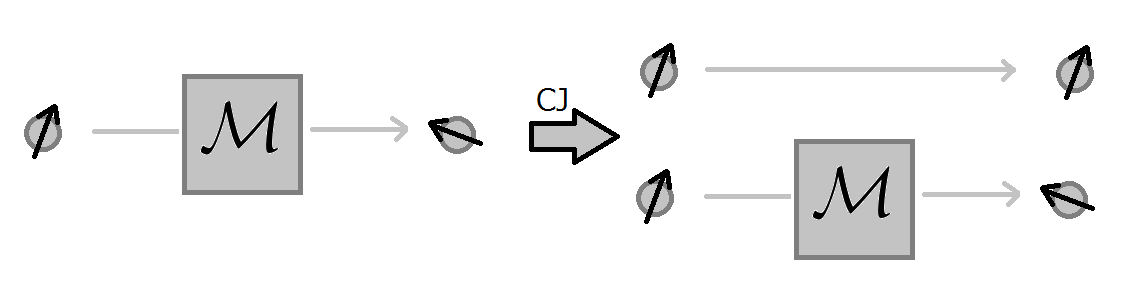
\includegraphics[width=0.8\textwidth]{obrazki/cj_new}
\caption{Rysunek ilustruje działanie izomorfizmu CJ. Zamiast działać odwzorowaniem na pewien stan izomorfizm CJ pokazuje działanie na maksymalnie splątane cząstki. Z powodu izomorfizmu w drugą stronę, konwencjonalnie interpretuje się izomorfizm CJ jako teleportacje bramek kwantowych.}
\end{figure}
\begin{definicja}
Macierz CJ $M^{A_1A_2}_i \in \Mats{\Hx{A_1} \otimes \Hx{A_2}} \geq 0$ odwzorowania CP $\mathcal{M}: \mathcal{L}(\Hx{A_1}) \mapsto \mathcal{L}(\Hx{A_2})$ definiuje się następująco:
\begin{gather}
\label{eq:cj_iso}
\MCJ(\mathcal{M^A}_i)= M^{A_1A_2}_i := [\mathcal{I} \otimes \MAi{ \KKet{\I} \BBra{\I}}]^T= \left[\sum^{d_{A_1}-1}_{i,j=0} \Ket{i}\Bra{j} \otimes \mathcal{M}^A_i(\Ket{i}\Bra{j})\right]^T, \\
\KKet{\I} = \sum^{d_{A_1}-1}_{i=0} \Ket{ii},
\end{gather}
gdzie $\{\Ket{j}\}^{d_{A_1}}$ tworzy ortonormalna bazę w $\HAi$. 
\end{definicja}
Często wygodnie korzystać z odpowiednika \eqref{eq:id_proj0} i \eqref{eq:id_proj} dla postaci CJ odwzorowań, który wygląda następująco:
\begin{gather}
\Trs_{A_2} \left[ M^{A_1A_2}_i \right] \leq \I^{A_1},~\forall i\\ 
\sum_i \Trs_{A_2} \left[ M^{A_1A_2}_i \right] = \I^{A_1}
\end{gather}
\begin{definicja}
Drugi izomorfizm CJ pozwala przedstawiać macierze przy pomocy wektorów, tzw. "podwójnych ketów". Wektor CJ macierzy A zdefiniowany jest jako
\begin{equation}
\KKet{A} := \I \otimes A\KKet{\I} = \sum^{d_{A_1}-1}_{i=0} \Ket{i} A \Ket{i}
\end{equation}
\end{definicja}
Znajomość izomorfizmów CJ pozwala na wprowadzenie macierzy procesu.
\begin{definicja}
Dwustronną macierzą procesu nazywa się taką macierz $W  \in \Mats{\Hx{A_1} \otimes \Hx{A_2} \otimes \Hx{B_1} \otimes \Hx{B_2}}$, która spełnia warunki
\begin{gather}
\label{eq:non_neg}
\WAll \geq 0. \\
\label{norm}
\Trs \WAll = d_{A_2B_2} \\
\label{eq:sums_to_id1}
\Trs
\left[
\WAll
\left(
M^{A_1A_2} \otimes M^{B_1B_2}
\right)
\right]=1.\\
\label{eq:sums_to_id2}
\forall M^{A_1A_2}, M^{B_1B_2} \geq 0, \Trs_{A_2} \MA = \mathbb{1}^{A_1}, \Trs_{B_2} \MB = \mathbb{1}^{B_1},
\end{gather}
gdzie $\MA = \sum_i \mai{i}$. W celu wyliczenia prawdopodobieństw zawartych w macierzy procesu korzysta się z następującej formuły:
\begin{equation}
\label{eq:cj_prob}
\Prt{\MAin}{\MXin{B}{j}} = \Tr{\WAll(M^{A_1A_2}_i \otimes M^{B_1B_2}_j)}.
\end{equation}
\end{definicja}
Warunek \eqref{eq:non_neg} zapewnia, że prawdopodobieństwa nie będą ujemne, a \eqref{eq:sums_to_id1} i  \eqref{eq:sums_to_id2} - pewność zaobserwowania dowolnej pary odwzorowań. 
%tutej moze macierz gestosci
%\begin{figure}[t]
%\centering

%\begin{tabular}{|c|c|c|c|}
%\hline
%Przyczynowy porządek & Stany & Kanały & Kanały z pamięcią \\
%\hline
%$A \npreceq B $ & $A_1, B_1, A_1B_1$ & $A_1B_2$ & $A_1B_1B_2$\\
%\hline
%$B \npreceq A $ & $A_1, B_1, A_1B_1$ & $A_2B_1$ & $A_1A_2B_1$\\ 
%\hline
%& \includegraphics[width=0.2\textwidth]{obrazki/states} & %\includegraphics[width=0.2\textwidth]{obrazki/channel}& \includegraphics[width=0.2\textwidth]{obrazki/channel_with_memory}\\
%\hline
%\end{tabular}
%\caption{Wyrażenia zgodne z formalizmem i ich proponowana graficzna interpretacja}
%\label{fig:configs}
%\end{figure}
W celu dalszej analizy macierzy procesu wygodne jest wprowadzenie bazy Hilberta-Schmidta.
\begin{definicja}
Baza Hilberta-Schmidta dla $\LHx{X}$ dana jest przez zbiór macierzy $\{\sigma^X_\mu\}^{d^2_X-1}_{\mu=0},$ gdzie $\sigma^X_0 = \mathbb{1}, \Tr{\sigma^X_\mu\sigma^X_\nu}=d_x\delta_{\mu\nu}, \Tr{\sigma^X_{\mu>0}}=0.$ Ogólny element przestrzeni $\Mats{\Hx{A_1}\otimes\Hx{A_2}\otimes\Hx{B_1}\otimes\Hx{B_2}}$ można zapisać, jako
\begin{gather}
\WAll = \sum_{\mu\nu\lambda\gamma} w_{\mu\nu\lambda\gamma} \sigma_\mu^{A_1}\otimes\sigma_\nu^{A_2}\otimes\sigma_\lambda^{B_1}\otimes\sigma_\gamma^{B_2} \\
w_{\mu\nu\lambda\gamma} \in \mathcal{C} \nonumber.
\end{gather}
\end{definicja}
Wyrażenia zawierające wyłącznie wyrazy $\sigma^{A_1}_i \otimes \mathbb{1}^{reszta},~(i > 0)$ nazywa się wyrażeniami typu $A_1$, wyrażenia zawierające  $\sigma^{A_1}_i \otimes \sigma^{A_2}_j \otimes \mathbb{1}^{reszta},~(i, j > 0)$ nazywa się wyrażeniami typu $A_1A_2$ etc.
Najogólniejsza macierz procesu generująca prawidłowe prawdopodobieństwa, tak długo jak jest dodatnia, dla odwzorowań zgodnych z \eqref{eq:non_neg} i \eqref{eq:sums_to_id1} to:
\begin{gather}
\WAll = \frac{1}{d_{A_1}d_{B_1}}(\mathbb{1} +\sigma^{B \preceq A} + \sigma^{A \preceq B} + \sigma^{A \npreceq \nsucceq B}) \\
\sigma^{A \preceq B} := \sum_{ij>0} a_{ij} \sigma^{A_1}_i \sigma^{B_2}_j + \sum_{ijk>0} b_{ijk} \sigma^{A_1}_i \sigma^{B_1}_j \sigma^{B_2}_k \\
\sigma^{B \preceq A} := \sum_{ij>0} c_{ij} \sigma^{A_2}_i \sigma^{B_1}_j + \sum_{ijk>0} d_{ijk} \sigma^{A_1}_i \sigma^{A_2}_j \sigma^{B_1}_k \\
 \sigma^{A \nprec \nsucc B} := \sum_{i>0} e_i  \sigma^{A_1} + \sum_{i>0} f_i  \sigma^{B_1} + \sum_{ij>0} h_{ij} \sigma^{A_1}_i \sigma^{B_1}_j \\
 \forall_{ij} a_{ij}, b_{ij}, c_{ij}, d_{ij}, e_{ij}, f_{ij}, g_{ij}, h_{ij} \in \mathcal{R} \nonumber,
\end{gather}
gdzie $\sigma^{A \preceq B}$ można uznać za zasób, w którym Alicja znaduje się w przeszłości Boba, $\sigma^{B \preceq A}$ za zasób, w którym Bob jest w przeszłości Alicji, zaś $\sigma^{A \nprec \nsucc B}$ za zasób, w którym Alicja i Bob nie komunikują się ze sobą. Słuszność takiej interpretacji utwierdzają interpretacje poszczególnych wyrazów, które składają się na poszczególne zasoby. Zostały one opisane dalej.
Wyróżnia się trzy rodzaje wyrażeń należących do rodziny macierzy przedstawionych powyżej.
\subsection{Stany}
\begin{figure}[h]
\centering
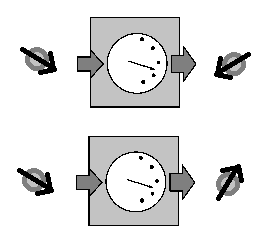
\includegraphics{obrazki/states_new}
\caption{Schematyczne przedstawienie stanów. Laboratoria wykonują pewne wybrane pomiary na systemach po czym wysyłają je ze swoich laboratoriów. Każde z laboratoriów otrzymuje różne, potencjalnie splątane, systemy.}
\end{figure}
Prawidłowe macierze procesu zawierające wyłącznie wyrazy typu $A_1 B_1, A_1, B_1$ produkują takie same statystyki jak macierze gęstości wraz z reguła Borna. 
Można więc intuicyjnie związać wyrazy typu $A_1 B_1, A_1, B_1$ z sposobem na opis stanów.
Do potwierdzenia powyższego twierdzenia w przypadku pomiarów rzutujących wykorzystuje się poniższe twierdzenie:
\begin{tw}
Macierz CJ, która opisuje zaobserwowanie pewnego stanu $\KP\BP$ i przygotowanie innego stanu $\Ket{\phi}\Bra{\phi}$ wygląda następująco:
\begin{equation}
\MCJ(\mathcal{M}) = \KP\BP \otimes \Ket{\phi}\Bra{\phi}^T.
\end{equation}
\end{tw}
W celu dowiedzenia powyższego twierdzenia zacząć można od przeanalizowania w jaki sposób wygląda postać mapy, która opisuje pomiar danego stanu $\Ket{\psi}$. Dobierając wektory $\{ \Ket{\psi_i} \}$ tak, by tworzyły bazę ortonormalną i $\Ket{\psi_0} = \Ket{\psi}$ z wcześniej podanej definicji działania mapy można zapisać:
\begin{equation}
\begin{split}
\mathcal{M}(\rho) &= \mathcal{M}\left(\sum_{ij} \alpha_{ij} \Ket{\psi_i}\Bra{\psi_j}\right) = \sum_{ijm} \left[ \alpha_{ij} E^\dag_m \Ket{\psi_i}\Bra{\psi_j}E_m\right]\\
&= \sum_{ijklefm} \left( {e_{lk}}_m {e_{ef}}_m^*\alpha_{ij} \Ket{\psi_k}\Bra{\psi_l} \Ket{\psi_i}\Bra{\psi_j} \Ket{\psi_e}\Bra{\psi_f}\right). 
\end{split}
\end{equation}
Biorąc pod uwagę fakt, że stan po otrzymana macierz po zadziałaniu mapą powinna być wielokrotnością $\Ket{\psi}$ (stan obserwowany jest z pewnym prawdopodobieństwem). Narzuca to warunek, że $k = 0$. Następnie zapisując regułę prawdopodobieństwa:
\begin{equation}
\Trs\left[ \mathcal{M}(\rho) \right] = \sum_{ijlk} \Trs \left[ {e_{0l}}_m{e_{0k}}_m^*\alpha_{ij} \Ket{\psi}\Bra{\psi_l} \Ket{\psi_i}\Bra{\psi_j} \Ket{\psi_k}\Bra{\psi}\right] =
\sum_{ijlkm} \Trs \left [ {e_{0l}}_m{e_{0k}}_m^*\alpha_{ij}\delta_{jk}\delta_{jl} \Ket{\psi}\Bra{\psi} \right] = \sum_{im} |{e_{0i}}_m| \alpha_{ii}.
\end{equation} 
Powyższy wynik musi się zgadzać z prawdopodobieństwem wynikającym z standardowej reguły prawdopodobieństwa, czyli:
\begin{equation}
\label{eq:a00}
\sum_{ij} \Trs \left[ \alpha_{ij} \Ket{\psi}\Bra{\psi} \Ket{\psi_i}\Bra{\psi_j}\right] = \sum_{j} \Trs \left[ \alpha_{0j} \Ket{\psi}\Bra{\psi_j} \right] = \alpha_{00}.
\end{equation}
Co narzuca warunek, że ${e_{ij}}_m = 0$ dla $i \neq 0 \land j \neq 0$. Jako, że pozostał wyłącznie wyraz typu $\Ket{\psi}\Bra{\psi}$ można dokonać sumowania po $m$ co daje:
\begin{equation}
\sum_{im} |{e_{00}}_m| \alpha_{ii} = \sum_{m} |e_{00}|_m \alpha_{ii} = e_{00} \alpha_{ii}.
\end{equation}
Korzystając ponownie z \eqref{eq:a00} widać, że $|e_{00}| = 1$.
Korzystając z definicji, postać CJ tego odwzorowania to:
\begin{equation}
\begin{split}
\MCJ(\mathcal{M}) &= \sum_{ij} \Ket{i}\Bra{j} \otimes (\Ket{\psi}\Bra{\psi}^\dag \Ket{j}\Bra{i} \Ket{\psi}\Bra{\psi})^T = \sum_{ij}\Ket{i}\Bra{j}  \otimes (\Ket{\psi}\left(\sum_l \beta_{l}^* \Bra{l}\Ket{j}\right)\left(\sum_k\beta_k\Bra{i}\Ket{k}\right)\Bra{\psi})^T \\&=  \sum_{ij} \beta_i \beta_j^* \Ket{i}\Bra{i} \otimes \KP\BP^T = \KP\BP \otimes \KP\BP^T.
\end{split}
\end{equation} Dalej zauważając, ewolucja unitarna jest już zapisana w odpowiedniej formie oraz wybierając macierz unitarną jako
$U = \sum_i \Ket{\phi_i}\Bra{\psi_i}$, gdzie wektory $\{ \Ket{\phi_i} \}$ tworzą bazę ortonormalną, a $\Ket{\phi_0}$ jest wybranym stanem, który chce się przygotować, złożenie poprzedniej z poprzednią transformacją ma postać:
\begin{equation}
\Ket{\psi}\Bra{\psi}\otimes U \Ket{\psi}\Bra{\psi} U^\dag = \Ket{\psi}\Bra{\psi}\otimes \Ket{\phi}\Bra{\phi}.
\end{equation}
Co pokazuje, że rzeczywiście tak wygląda odwzorowanie CJ dla pomiaru i przygotowania stanu. 
Przyjmując teraz następująco postać macierzy procesu:
\begin{equation}
W = \rho^{A_1B_1} \otimes \I^{A_2} \otimes \I^{B_2},
\end{equation} która opisuje każdą macierz procesu zawierającą wyłącznie wybrane w tym rozdziale wyrazy. Zapisując regułe prawdopodobieństwa otrzymuje się
\begin{equation}
\begin{split}
\Pr(x,y) &= \Trs\left[ (\rho^{A_1B_1} \otimes \I^{A_2} \otimes \I^{B_2}) (\Ket{\psi_x}\Bra{\psi_x}^{A_1} \otimes \Ket{\psi_y}\Bra{\psi_y}^{B_1} \otimes \Ket{\phi_x}\Bra{\phi_x}^{A_2} \otimes \Ket{\phi_y}\Bra{\phi_y}^{B_2})\right] \\
&= \Trs\left[ \rho \Ket{\psi_x}\Bra{\psi_x}\otimes\Ket{\psi_y}\Bra{\psi_y} \otimes \Ket{\phi_x}\Bra{\phi_x}\otimes\Ket{\phi_y}\Bra{\phi_y}\right] \\
&= \Trs\left[ \rho \Ket{\psi_x}\Bra{\psi_x}\otimes\Ket{\psi_y}\Bra{\psi_y}\right] \Trs\left[\Ket{\phi_x}\Bra{\phi_x}\right] \Trs\left[\Ket{\phi_y}\Bra{\phi_y}\right]
\\
&= \Trs\left[ \rho \Ket{\psi_x}\Bra{\psi_x}\otimes\Ket{\psi_y}\Bra{\psi_y}\right].
\end{split}
\end{equation}
Powyższe wyprowadzenie pokazuje, że dla pomiarów von Neumanna, tak zdefiniowana macierz procesu generuje takie same statystyki jak formalizm macierzy gęstości. Warto jeszcze zaznaczyć, że iloczynowa postać tej macierzy procesu zapewnia, że $\rho^{A_1B_1}$ również jest dodatnie, czyli spełnia wszystkie warunki narzucone przez formalizm macierzy gęstości. Jednym ze sposobów na pokazanie, że generowane są identyczne statystyki dla dowolnych POVM jest wykonanie jawnego rachunku:
\begin{equation}
\begin{split}
\Pr(x,y) &= \Trs\left[\rho^{A_1B_1} \otimes \I^{A_2B_2}(M_x^{A_1A_2}\otimes M_y^{B_1B_2})\right]\\ &=\sum_{ijkl}\Trs\left[( \alpha_{ijkl} \Ket{i}\Bra{j}^{A_1} \otimes \I^{A_2} \otimes \Ket{k}\Bra{l}^{B_1} \otimes \I^{B_2}) M_x^{A_1A_2} \otimes M_y^{B_1B_2}\right] \\ 
&= \sum_{ijklmnef} \Trs \left[ \alpha_{ijkl} \Ket{i}\Bra{j} \otimes \I \otimes \Ket{k}\Bra{l} \otimes \I)(\Ket{m}\Bra{n} \otimes \mathcal{M}_x(\Ket{n}\Bra{m})^T \otimes \Ket{e}\Bra{f} \otimes \mathcal{M}_y(\Ket{f}\Bra{e})^T \right] \\
&= \sum_{ijklmnef} \Trs \left[ \alpha_{ijkl} \Ket{i}\Bra{j}\Ket{m}\Bra{n}^{A_1} \otimes \Ket{k}\Bra{l}\Ket{e}\Bra{f}^{B_1} \right] \Trs\left[{\mathcal{M}_x(\Ket{n}\Bra{m})^{A_2}}^T \otimes {\mathcal{M}_y(\Ket{f}\Bra{e})^{B_2}}^T\right] \\
&= \sum_{mnef} \Trs \left[ \alpha_{ijkl} \Bra{n}\Ket{i}\Bra{j}\Ket{m} \otimes \Bra{f}\Ket{k}\Bra{l}\Ket{e}\right]\Trs\left[{\mathcal{M}_x(\Ket{n}\Bra{m})^{A_2}}^T \otimes {\mathcal{M}_y(\Ket{f}\Bra{e})^{B_2}}^T\right] \\
&= \sum_{mnef} \Trs\left[\alpha_{nmfe} \right] \Trs\left[{\mathcal{M}_x(\Ket{n}\Bra{m})^{A_2}}^T \otimes {\mathcal{M}_y(\Ket{f}\Bra{e})^{B_2}}^T\right] \\
&= \sum_{mnef} \Trs\left[\alpha_{nmfe}{\mathcal{M}_x(\Ket{n}\Bra{m})^{A_2}}^T \otimes {\mathcal{M}_y(\Ket{f}\Bra{e})^{B_2}}^T\right] \\
&= \Trs \left[ \mathcal{M}_x \otimes \mathcal{M}_y(\sum_{nmfe}\alpha_{nmfe} \Ket{n}\Bra{m} \otimes \Ket{f}\Bra{e})^T\right] \\
&= \Trs \left[  \mathcal{M}_x \otimes \mathcal{M}_y(\rho)^T\right] \\
&= \Trs \left[ \mathcal{M}_x \otimes \mathcal{M}_y(\rho)\right].
\end{split}
\end{equation}
Ostateczna postać po przekształceniach zgadza się z tą, która opisuje statystyki pomiarów na systemie złożonym opisywanym przez równanie \eqref{eq:probqi}. 
%Korzystając z tej wiedzy dla przypadku, w którym po pomiarze porzuci się system, lub równoważnie przyjmie się, że przestrzeń wyjściowa jest trywialna to powyższe odwzorowanie to $\KP\BP$. Pisząc dalej regułę prawdopodobieństwa
%\begin{equation}
%\Pr(x,y) = \Trs \left[ W \left(\Ket{\psi_x}\Bra{\psi_x} \otimes \Ket{\phi_y}\Bra{\phi_y}\right)\right].
%\end{equation} 
%Powyższe równanie można rozumieć tak, że dla pewnych projektorów $\KP\BP$ macierz W przypisuje im pewne statystyki pomiarowe. Również warunki  jakie wprowadzono na poprawność macierzy $W$ jest taka sama, jak ta którą wprowadzono na macierze procesu. Co wraz z faktem, że każda obserwable można rozpisać na liniowe kombinacje pewnych projektorów pozwala interpretować W w takim przypadku jako macierz gęstości, a kombinację liniową projektorów jako obserwable. Przytaczając argument, że POVM można zrealizować unitarną ewolucją i pomiarem w więcej wymiarowej przestrzeni można rozszerzyć powyższy argument również na POVM co uzasadnia interpretacje wyrazów $A_1B_1$, jako macierzy gęstości. 
Przykładowo macierz procesu, która opisuje sytuację, gdzie laboratoria dzielą maksymalnie splątane
\footnote{Do sprecyzowania co rozumiane jest pod pojęciem maksymalnego splątania konieczne jest wprowadzenie miary splątania. Przez miarę splątania rozumie się taką funkcje, która jest monotoniczna, gdy laboratoria mogą wykonywać lokalne operacje i komunikować się klasycznie (np. telefonem). Konieczne również jest, by zbiegała do zera dla stanów niesplątanych. Przykładem takiej miary jest entropia von Neumanna definiowana przez $S(\rho) = -\Trs \left[ \rho \log \rho \right]$. Okazuje się, że jest ona maksymalna dla $\frac{1}{d}\KKet{\I}\BBra{\I}$ \cite{review}.
}
 cząsteczki zapisuje się następująco:
\begin{equation}
W = \KKet{\I}\BBra{\I}^{A_1B_1} \otimes \I^{A_2} \otimes \I^{B_2}.
\end{equation}

\subsection{Kanały}
\begin{figure}[h]
\centering
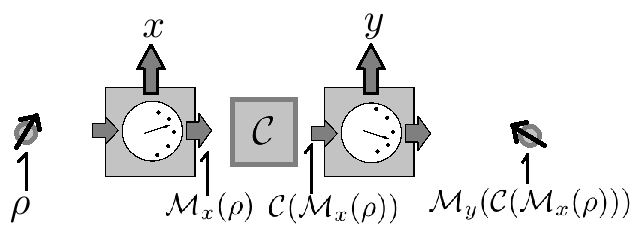
\includegraphics{obrazki/channel_new}
\caption{Schematyczna reprezentacja kanału CPTP. Alicja wykonuje wybrane operacje na systemie po czym wysyła go do Boba. W trakcie przesyłania systemu zostaje zaaplikowana unitarna transformacja $U$.}
\end{figure}
Wyrazy typu $A_2B_1$, $B_2A_1$ identyfikuje się jako sposób opisywania kanałów, ze względu na występowanie tych wyrazów w macierzach CJ kanałów.
Łatwo zaobserwować, że formuła
\begin{equation}
\Trs \left[ \mathcal{M}_y^B \circ \mathcal{C} \circ \mathcal{M}_x^A(\rho)\right]
\end{equation} opisuje statystyki pomiarowe eksperymentu, w którym Alicja wykonuje pewne pomiary przesyła system kanałem CPTP $\mathcal{C}$ po czym Bob wykonuje swoje pomiary na otrzymanym systemie to nie oczywista jest jej równoważność z 
\begin{equation}
\Trs \left[\left( \rho^{A_1}\otimes  {C^{A_2B_1}}^T \otimes \I^{B_2}\right)(M_x^{A_1A_2}\otimes M_y^{B_1B_2})\right].
\end{equation} Można to pokazać następująco: 
\begin{equation}
\begin{split}
\Trs&\left[ \left(\rho^{A_1} \otimes C^{A_2B_1} \otimes \I \right)\left(M_x^{A_1A_2}\otimes M_y^{B_1B_2}\right)\right] \\
&= \sum_{ijklmn} \Trs \left[ \left(\rho \otimes \Ket{i}\Bra{j} \otimes \mathcal{C}(\Ket{i}\Bra{j}) \otimes \I\right)\left(\Ket{k}\Bra{l} \otimes \mathcal{M}_x(\Ket{l}\Bra{k})^T \otimes \Ket{m}\Bra{n} \otimes \mathcal{M}_y(\Ket{n}\Bra{m})^T\right)\right] \\
&= \sum_{ijklmn} \Trs \left[ \rho \Ket{k}\Bra{l} \otimes \Ket{i}\Bra{j}\mathcal{M}_x(\Ket{l}\Bra{k})^T \otimes \mathcal{C}(\Ket{i}\Bra{j})\Ket{m}\Bra{n} \otimes \mathcal{M}_y(\Ket{n}\Bra{m})^T\right] \\
&= \Trs\left[\rho\Ket{k}\Bra{l}\right] \Trs\left[\Ket{i}\Bra{j}\mathcal{M}_x(\Ket{l}\Bra{k})\right] \Trs\left[\mathcal{C}(\Ket{i}\Bra{j}) \Ket{m}\Bra{n}\right] \Trs\left[\mathcal{M}_y(\Ket{m}\Bra{n})\right] \\
&= \sum_{ijmn}  \Trs\left[\Ket{i}\Bra{j}\mathcal{M}_x(\sum_{lk} \rho_{lk} \Ket{l}\Bra{k})^T\right] \Trs\left[\mathcal{C}(\Ket{i}\Bra{j}) \Ket{m}\Bra{n}\right] \Trs\left[\mathcal{M}_y(\Ket{n}\Bra{m})^T\right] \\
&= \sum_{ijmn}  \Trs\left[\Ket{i}\Bra{j}\mathcal{M}_x(\rho)^T\right] \Trs\left[\mathcal{C}(\Ket{i}\Bra{j}) \Ket{m}\Bra{n}\right] \Trs\left[\mathcal{M}_y(\Ket{n}\Bra{m})^T\right] \\
&= \sum_{mn} \Trs \left[ \mathcal{C}(\mathcal{M}_x(\rho))\Ket{m}\Bra{n}\right]\Trs\left[\mathcal{M}_y(\Ket{n}\Bra{m})^T\right] \\
&=  \Trs\left[ \mathcal{M}_y (\mathcal{C}(\mathcal{M}_x(\rho)))^T\right] = \Trs\left[ \mathcal{M}_y (\mathcal{C}(\mathcal{M}_x(\rho)))\right] \\
&=\Trs \left[ \mathcal{M}_y^B \circ \mathcal{C} \circ \mathcal{M}_x^A(\rho)\right]
\end{split}
\end{equation}
Przykładowo macierz opisująca odwracalny kanał, który wysyła cząstkę z $A_2$ do $B_1$ i wykonuje pewna operację unitarną U to $\KKet{U}\BBra{U}^{A_2B_1}$. Korzystając z wcześniej opisanej detekcji stanu i przygotowania innego stanu eksperyment, w którym Alicja wysyła system zakodowany w bazie $z$, a Bob wykonują pomiar w bazie $z$ następnie Alicja przesyła dalej swój system, a Bob przesyła stan maksymalnie zmieszany stan 
($\frac{1}{2}\I$) można opisać następującymi odwzorowaniami
\begin{gather}
\xi(i) = \Ket{i}\Bra{i} \otimes \Ket{i}\Bra{i} \\
\eta(j) = \Ket{j}\Bra{j} \otimes \frac{1}{2}\I.
\end{gather} 
W celu skrócenia zapisu pominięto indeksy górne, które pozostaną dalej niejawne, gdy ich brak nie będzie wprowadzał niejasności.
Można się spodziewać, że gdy laboratoria będzie łączył kanał z $A_2$ do $B_1$, który zamienia $\Ket{i} \mapsto \Ket{i \oplus 1}$, kanał ten opisuje postać CJ macierzy unitarnej $\sum_i \Ket{i}\Bra{i \oplus 1}$, a Alicja na wejściu dostaje stan maksymalnie zmieszany, to prawdopodobieństwo
zaobserwowania stanu $\Ket{j}$ u Boba będzie równe $1$, gdy Alicja wyśle mu stan $\Ket{j \oplus 1}$ i zerowe w przeciwnym wypadku. Podejrzenia te potwierdza jawny rachunek:
\begin{gather}
W = \sum_{ijkl} \I \otimes \Ket{i}\Bra{j} \otimes \Ket{k\oplus 1}\Bra{k} \Ket{i}\Bra{j} \Ket{l}\Bra{l \oplus 1} \otimes \I \\
\begin{split}
\Pr(i,j) &= \frac{4}{\Trs W} \Trs\left[ W (\xi(i) \otimes \eta(j))\right]\\&=C \sum_{efkl} \Trs [\I \otimes \Ket{e}\Bra{f} \otimes \Ket{k\oplus 1}\Bra{k} \Ket{e}\Bra{f} \Ket{l}\Bra{l \oplus 1} \otimes \I)(\Ket{i}\Bra{i} \otimes \Ket{i}\Bra{i} \otimes \Ket{j}\Bra{j} \otimes \I)] \\
&= \frac{2}{8} \sum_{efkl} \delta_{if} \delta_{j(l \oplus 1)} \Trs \left[ \Ket{i}\Bra{i} \otimes \Ket{e}\Bra{i} \otimes \Ket{k \oplus 1}\Bra{k}\Ket{e}\Bra{f}\Ket{l}\Bra{j} \otimes \I \right] \\
&= \frac{2}{8} \sum_{efkl} \delta_{if} \delta_{ke} \delta_{fl} \delta_{j(l \oplus 1)} \Trs \left[ \Ket{i}\Bra{i} \otimes \Ket{e}\Bra{i} \otimes \Ket{k \oplus 1} \Bra{j} \otimes \I\right] \\
&= \frac{2}{8} \sum_{k} \delta_{i(j \oplus 1)} \Trs \left[ \Ket{i}\Bra{i} \otimes \Ket{k}\Bra{i} \otimes \Ket{k \oplus 1}\Bra{j} \otimes \I \right]  \\
&= \frac{2}{8} \sum_k \delta_{i(j \oplus 1)} \Trs \left[ \Ket{i}\Bra{i} \otimes \Ket{k}\Bra{i} \otimes \Ket{k \oplus 1}\Bra{i \oplus 1} \otimes  \I\right] \\
&=  \frac{1}{2} \delta_{i(j \oplus 1)}.
\end{split} 
\end{gather}  Co potwierdza podejrzenia, że powyższy zasób jest kanałem od Alicji do Boba.
\subsection{Kanały z pamięcią}
\begin{figure}[h]
\centering
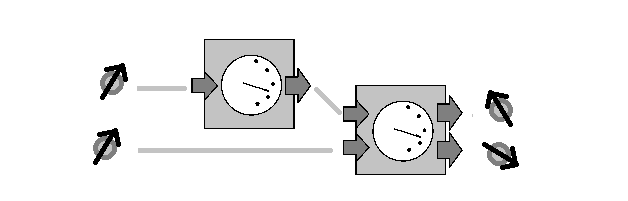
\includegraphics{obrazki/memory_new}
\caption{Schematyczna reprezentacja kanału z pamięcią na przykładzie zasobu wykorzystywanego do implementacji kodowania supergęstego. Alicja z Bobem dzielą maksymalnie splątane cząstki. Alicja wykonuje pewną unitarną transformacje i wysyła swój system dalej do Boba.}
\end{figure}
Do opisywania kanałów z pamięcią wykorzystuje się wyrazy typu $B_1B_2A_1$, $A_1A_2B_1$. Są one najogólniejszym wyrazem zgodnym wymaganiami narzuconymi na macierze procesu.
Ciekawym przykładem kanału z pamięcią może być zasób wykorzystywany przy implementacji kodowania supergęstego (\textit{superdense coding}). Jest to protokół, który wykorzystuje się do przesłania dwóch bitów informacji od Alicji do Boba. Początkowo produkowana jest para maksymalnie splątanych cząsteczek jedna jest wysłana do Alicji druga do Boba. Następnie Alicja wykonuje jedną z czterech lokalnych unitarnych transformcji na swoim systemie po czym wysyła swój system do Boba. Macierze, którymi działa Alicja to 
$\{ U_i\}=\{ \I, \X, \Z, -i\Y \}$, gdzie $\X, \Y, \Z$ to macierze Pauliego:
\begin{equation}
\X = \begin{pmatrix}
0 &1\\
1 &0
\end{pmatrix}~
\Y = \begin{pmatrix}
0 &-i\\
i &0
\end{pmatrix}~
\Z = \begin{pmatrix}
1 &0\\
0 &-1
\end{pmatrix}.~
\end{equation} Okazuje się, że po wykonaniu lokalnej transformacji system złożony znajduje się w jednym z czterech ortogonalnych stanów, co pozwala Bobowi, po otrzymaniu systemu od Alicji, określić jaką transformację wykonała Alicja, czyli otrzymać wiadomość od Alicji zakodowaną w wykonanej przez nią transformacji. Wyjątkowość tego protokołu polega na fakcie, że Bob może otrzymać pierwszą cząstkę arbitralnie wcześniej, niż
cząstkę, którą otrzyma od Alicji, co więcej może on otrzymać tą cząstkę zanim Alicja zdecyduje jakie 2 bity chce mu przesłać. Co może błędnie sugerować, że Alicja wysłała dwa klasyczne bity przy pomocy jednego kubitu. Sytuacja taka jest zabroniona przez granicę Holevo (\textit{Holevo bound}). Mimo wszystko dwa kubity są wysyłane w celu przesłania dwóch klasycznych bitów co nie wprowadza sprzeczności.
W celu wykonania tego protokołu potrzebne są dwie maksymalnie splątane cząsteczki i kanał od Alicji do Boba. Korzystając z wiedzy z poprzednich dwóch podrozdziałów zapisuje się ten zasób następująco:
\begin{equation}
W = \KKet{\I}\BBra{\I}^{A_1B_{11}}\KKet{\I}\BBra{\I}^{A_2B_{12}} \I^{B_{21}B_{22}},
\end{equation} gdzie w tym przypadku Bob operuje na dwóch cząstkach. W przypadku Boba pierwsza cyfra indeksów dolnych systemów Boba wskazuje, czy dany system jest wejściowy czy wyjściowy, zaś druga cyfra jest porządkowa.
Stany po wykonaniu kolejnych unitarnych transformacji z dokładnością do stałej to $\{ \Ket{\psi_i} \}$ = $\{\I \otimes U_i \Ket{\psi_i} \}$ = $\{ \Ket{00} + \Ket{11}, \Ket{10} + \Ket{01}, \Ket{00} - \Ket{11}, \Ket{10} - \Ket{01}\}$.
Postać CJ operacji wykonywanych przez poszczególne strony to:
\begin{gather}
\xi(i) = \frac{1}{4} \sum_{ef} \Ket{e}\Bra{f} \otimes U_i \Ket{e}\Bra{f} U_i^\dag  \\
\eta(j) = \frac{1}{4} \Ket{e}\sum_{ef} U_j \Ket{e}\Bra{f} U_j^\dag\Bra{f} \otimes \I.
\end{gather} Korzystając z reguły prawdopodobieństwa i zapisując systemy w kolejności $A_{1} A_2 B_{11} B_{12} B_{21} B_{22}$ wykonuje się następujące obliczenia:
\begin{gather}
\begin{split}
\Pr&(j|i) = \frac{1}{2}\Trs \left[ W (\xi(i) \otimes \eta(j)\right] \\
 &= \frac{1}{32}\sum_{efklmnqp} \Trs \left[\Ket{e}\Bra{f} \otimes \Ket{k}\Bra{l} \otimes \Ket{e}\Bra{f} \otimes  \Ket{k}\Bra{l} \otimes \I \otimes \I \left( \Ket{m}\Bra{n} \otimes U_i\Ket{m}\Bra{n}U_i^\dag \otimes \Ket{q}U_j\Ket{q}\Bra{p}\Bra{p}U_j^\dag\otimes \I\otimes \I\right)\right] \\
 &= C\sum_{efklmnqp} \delta_{fm}
\delta_{l(m + (i \oplus 1) \oplus 1)}
\delta_{fq} 
\delta_{l(q + (j \oplus 1) \oplus 1)} \Trs \left [ \Ket{e}\Bra{n} \otimes \Ket{k}\Bra{n}U_i^\dag\otimes \Ket{e}\Bra{p} \otimes \Ket{k}\Bra{p}U_j^\dag \otimes \I \otimes \I\right] \\
&=4C \sum_{efkmnqp} \delta_{(m + (i \oplus 1) \oplus 1)(q + (j \oplus 1) \oplus 1)} \delta_{fm} \delta_{fq} \Trs \left [ \Ket{e}\Bra{n} \otimes \Ket{k}\Bra{n}U_i^\dag\otimes \Ket{e}\Bra{p} \otimes \Ket{k}\Bra{p}U_j^\dag \right] \\
&= 4C \sum_{ekmnp} \delta_{(i \oplus 1)(j \oplus 1)} \Trs \left [ \Ket{e}\Bra{n} \otimes \Ket{k}\Bra{n}U_i^\dag\otimes \Ket{e}\Bra{p} \otimes \Ket{k}\Bra{p}U_j^\dag \right] \\
&= \delta_{ij}
\end{split} \nonumber\\
C = \frac{-1^{(i \div 2 + j \div 2)}}{32}
\end{gather} gdzie powyżej $x \oplus y$ traktowano jako $x + y \mod 2$, zaś $\div$ to dzielenie bez reszty. Powyższe obliczenia pokazują, że rzeczywiście opisywany jest tutaj protokół supergęstego kodowania.
%Ponownie w celu skrócenia pozostawiono iloczyn tensorowy niejawnym, który dalej również będzie pomijany, gdy będzie on indukowany przez jego pozycję.
\section{Przyczynowa separowalność i przyczynowe nierówności}
\begin{definicja}
Macierzami procesu \textit{causally separable} (przyczynowo separowalnymi) nazywa się takie macierze, które można zapisać jako wypukłą kombinację procesów o implementowalnych przy założeniu określonej struktury przyczynowej:
\begin{equation}
\label{eq:sep}
\WAll = qW^{B \nprec A} + (1-q)W^{A \nprec B},~0 \leq q \leq 1,
\end{equation}
gdzie
\begin{gather}
W^{B \nprec A} := \frac{1}{d_{A_1}d_{B_1}}\I + \sigma^{A \preceq B} + \sigma^{A \npreceq \nsucceq B} \\
W^{A \nprec B} := \frac{1}{d_{A_1}d_{B_1}}\I + \sigma^{B \preceq A} + \sigma^{A \npreceq \nsucceq B} \\
W^{A \nprec \nsucc B} := \frac{1}{d_{A_1}d_{B_1}}\I + \sigma^{A \nprec \nsucc B},
\end{gather}
\end{definicja}
Pierwszą rodzinę procesów można interpretować jako zasób, w którym Bob nie jest przed Alicja, a drugi jako ten, w którym Alicja nie jest przed Bobem.
Powyższa dekompozycja nie musi być jednoznaczna, jako że wyrazy typu $W^{A \nprec \nsucc B}$ można włączyć do wybranego wyrazu.
Przed wprowadzeniem przyczynowej nierówności (\textit{causal inequallity}) warto wspomnieć o tzw. nierówności Bella. Jest to nieskończona rodzina nierówności, których żaden niesplątany system nie może złamać. Jest to niezależny od implementacji pomiarów (\textit{device independent}) sposób weryfikacji splątania kwantowego. 
\begin{definicja}
Nierówność przyczynowa to taka nierówność wynikająca z pewnego zadania komunikacyjnego, która ogranicza wyniki jakie można osiągnąć w danym zadaniu korzystając z zasobów przyczynowych. Niespełnianie takiej nierówności implikuje fakt, że dany zasób jest nieprzyczynowy.
\end{definicja}
Przykład takiej nierówności przedstawiony jest poniżej.
%%Typowym przykładem jest eksperyment, w którym w środkowym punkcie pomiędzy odległymi laboratoriami
%przygotowuję się dwie cząsteczki i wysyła się po jednej cząstce do każdego z laboratoriów po pierwsza strona, tradycyjnie nazywana Alicją, wykonuje jeden pomiar zwracający jakiś binarny wynik $A_n$ przyjmujący wartości $\pm 1$, następnie wykonuje po raz kolejny pomiar potencjalnie 
%nierówności wynikająca z analizy następującej funkcji zmiennych losowych
%\begin{gather}
%g_n = A_nB_n+ A'_nB_n + A_nB'_n + A'_n+B'_n
%\end{gather}
%\end{multicols*}
Przyjmuje się następujące założenia na temat natury rzeczywistości uporządkowanej przyczynowo:
\begin{description}
	\item[Przyczynowa struktura (\textit{causal structure}, CS)]
	Wydarzenia obdarzone są częściowym porządkiem w strukturze czasoprzestrzeni, można wyznaczyć kolejność wydarzeń $A \prec B$, która wyznacza kierunek przesyłania informacji; jeżeli $A \prec B$, to możliwe jest sygnalizowanie
	\footnote
	{W przypadku, gdy $A \prec B$ oznacza to, że brzegowy rozkład prawdopodobieństwa otrzymania danego wyniku nie zależy od wejścia drugiej strony. $\Pr(a|x, y) = \Pr(a|x, y')~\forall a,x,y,y'$, $\Pr(a|x,y) = \sum_b \Pr(a,b|x,y)$, gdzie przez a, b oznaczamy wyniki otrzymane przez odpowiednie strony, zaś x, y ich wejścia.} 
	z A do B, lecz nie na odwrót.
	\item[Wolny wybór (\textit{Free choice}, FC)]  
	W przypadku wyboru liczb losowych, możliwe korelacje występują wyłącznie z wynikami z przyszłości.
	\item[Zamknięte laboratoria (\textit{Closed laboratories}, CL)] 
	Liczba odgadnięta przez Alicję może być skorelowana z liczbą losową Boba wyłącznie, jeżeli system wysłany do Alicji jest przed (w sensie przyczynowości) generacją liczby Boba, analogicznie w przypadku odwrotnym.	
\end{description}
Rozważa się następująca dwustronną grę realizowaną wielokrotnie przez dwa odległe laboratoria (Alicję i Boba). W każdej iteracji rozgrywki Alicja i Bob otrzymują na wejściu pewien fizyczny system, wykonują na nim pewne operacje i wysyłają dalej system. Każda ze stron może otrzymać sygnał wyłącznie przez 
system wchodzący do laboratorium, zaś wysłać wyłącznie przez system wychodzący z laboratorium. Widać więc, że jeżeli Alicja otrzyma system, który przeszedł pewną procedurę u Boba, to Bob może wysłać informacje, zaś Alicja może ją wyłącznie odebrać, co uniemożliwia dwustronna sygnalizację.
Każdy z graczy otrzymując system losuje jeden bit wybraną metodą oznaczany a dla Alicji i b dla Boba. Dodatkowo Bob losuje bit b', który decyduje, czy Bob ma zgadywać bit $a$ Alicji, czy Alicja ma zgadywać bit $b$ Boba. Bez utraty ogólności można przyjąć, że obie strony zgadują bit drugiego gracza. W zależności od b' ich 
predykcja może się nie liczyć. Zakłada się, że bity losowane są z równym prawdopodobieństwem. Prawdopodobieństwo sukcesu w takiej grze zapisuje się następująco
\begin{equation}
\Pr{}_{sukcesu} := \frac{1}{2} \left[ \Pr(x=b|b'=0) + \Pr(y=a|b' = 1)\right]
\end{equation}
Każda strategia w uporządkowanej strukturze czasu osiąga $\Pr{}_{sukcesu} \leq \frac{3}{4}$. Optymalna strategie opisuje się nierygorystycznie następująco: w przypadku $A \prec B$ Alicja może zakodować swój bit w pewien sposób w systemie, który wyśle do Boba, dlatego można wybrać taką strategię, że $\Pr(y=a) = 1$, Alicji pozostaje wtedy losowa predykcja co do wartości bitu Boba - $\Pr(x=b) = \frac{1}{2}$. Można również pokazać, że żadna probabilistyczna strategia nie może poprawić wyniku, co daje optymalną strategię. Okazuje się, że korzystając z korelacji opisywanych przez formalizm macierzy procesu $\Pr{}_{sukces} \leq \frac{2+\sqrt{2}}{4}$.
Można rozważyc następującą macierz procesu
\begin{equation}
\WAll = \frac{1}{4}\left[
\I\I\I\I + \frac{1}{\sqrt{2}}(\I\Z\Z\I + q\Z\I\X\Z + \frac{(1-q)}{2}\Z\I\X\I)
\right],~ 0 \leq q \leq 1.
\end{equation}
Macierze $\I, \X, \Y, \Z$ tworzą bazę Hilberta-Schmidta. W powyższym zapisie pominięto iloczyn tensorowy, w celu skrócenia zapisu w miejscach, gdzie jego brak nie powinien wprowadzać nieporozumień - $\I^{A_1}\X^{A_2}\Y^{B_1}\Z^{B_2} =: \I\X\Y\Z$.
Przedstawioną macierz z $q=1$ wraz z dalej przedstawioną procedurą komunikacji wprowadzono w \cite{process_matrix} jako zasób, który pozwala złamać przyczynową nierówność wynikającą z tej gry. W \cite{max_violation} pokazano, że przy odpowiednich założeniach o dozwolonych operacjach jest to maksymalne przekroczenie nierówności
wynikającej z tego zadania. Z drugiej strony widać od razu, że przy $q=0$ mamy $A \prec B$, zatem oczywistym jest, że taki zasób nie pozwala złamać przyczynowej nierówności. Sterując wartością $q$ można zaobserwować odpowiednio przejścia macierzy z ustalonej przyczynowości poprzez separowalną do nieseparowalnej.
Macierze separowalne nie mogą łamać żadnej nierówności przyczynowej, nieseparowalne zostaną dokładniej opisane dalej. Procedura komunikacji wygląda następująco. 
Za każdym razem Alicja mierzy swój system w bazie $z$ i przypisuje $x = 0$ dla $\Ket{z_+}$ zaś $x=1$ dla $\Ket{z_-}$, a następnie przygotowuje na nowo kubit i zakodowuje a w tej samej bazie. Odwzorowanie CP Alicji wygląda następująco:
\begin{equation}
\xi(x, a) = \frac{1}{4}
\left[
\I + (-1)^x \Z
\right]
\otimes
\left[
\I  + (-1)^a \Z
\right	].
\end{equation}
Natomiast, gdy Bob jako posiadacz bitu $b'$ chce odczytać bit Alicji, mierzy przychodzący kubit w bazie $z$i przypisuje wyniki tego pomiaru do y analogicznie jak Alicja. W tym przypadku nieistotne jest jaki stan przygotuje Bob, więc przygotowuje dowolny stan $\rho^{B_2}$ znormalizowany do $\Trs (\rho^{B_2}) = 1$.
W przypadku $b'=0$, Bob chce wysłać swój bit do Alicji. Dokonuje pomiaru w bazie x, następnie w przypadku wyniku $y = \Ket{x_+}$ zakodowuje swój bit następująco: $0 \to \Ket{z_+}, 1 \to \Ket{z_-}$ w drugim kodowanie wygląda odwrotnie $1 \to \Ket{z_+}, 0 \to \Ket{z_-}$. Jego odwzorowanie wygląda następująco
\begin{equation}
\eta(y, b, b') =
\begin{cases}
\frac{1}{2}\left[
\I + (-1)^y\Z
\right] \otimes \rho&b'=1\\
\frac{1}{4} \left[ \I + (-1)^y \X \right] \otimes \left[ \I + (-1)^{b+y} \Z \right]& \text{w przeciwnym wypadku}.
\end{cases}
\end{equation}
Przypominając, że prawdopodobieństwo sukcesu w tej grze dane jest jako
\begin{equation}
\Pr{}_{sukcesu} := \frac{1}{2} \left[ \Pr(x=b|b'=0) + \Pr(y=a|b' = 1)\right],
\end{equation}
i przyjmując dla wygody obliczeń, że $\rho$ w mapie Boba to $\frac{1}{2}\I$
\begin{equation}
\begin{split}
\Pr(x, y|a, b, 1)_q &= \frac{1}{4}\left(p_1 + p_2 + p_3 + p_4\right) \\
p_1 &= \frac{1}{16} \Trs \left[ \left( \I + (-1)^x\Z\right) \otimes \left( \I+(-1)^a\Z\right) \otimes \left(\I + (-1)^y \Z\right) \otimes \I\right] \\
&= 1 \\
p_2 &= \frac{1}{16\sqrt{2}} \Trs \left[ \I\Z\Z\I\left( \I + (-1)^x\Z\right) \otimes \left( \I+(-1)^a\Z\right) \otimes \left(\I + (-1)^y \Z\right) \otimes \left( \I + (-1)^{b+y}\Z\right)\right] \\
&= \frac{4}{16\sqrt{2}} \Trs \left[ \left( \Z +(-1)^a\Z\Z\right) \otimes \left( \Z + \Z\Z(-1)^y\right) \right] \\
&= \frac{1}{\sqrt{2}} (-1)^a (-1)^y \\
p_3 &= \frac{q}{8\sqrt{2}} \Trs \left[ \left( \Z + (-1)^x\Z\Z\right) \otimes (\X + (-1)^y \X\Z) \otimes \Z\right]\\
&= \frac{1}{4\sqrt{2}} (-1)^x ~0~0 \\
p_4 &= 0
\end{split}
\end{equation}
Co po obliczeniu odpowiednich rozkładów brzegowych i wykonaniu analogicznych obliczeń dla $b' = 0$ daje:
\begin{gather}
\Pr(x=b|b'=0)_q = \frac{\sqrt{2}q+2}{4} \\
\Pr(y=a|b'=1)_q = \frac{\sqrt{2}+2}{4} \\ 
\Pr{}_{sukcesu_q} = \frac{\sqrt{2}q + \sqrt{2} + 4}{8},
\end{gather}
gdzie indeks odnotowuje zależność prawdopodobieństwa od $q$. Tak jak się spodziewano, prawdopodobieństwo sukcesu Alicji rośnie wraz ze zwiększaniem współczynnika przy członie $\Z\I\X\Z$ rozumianym jako reprezentacja kanału kwantowego z pamięcią, który odpowiada za sygnalizujące korelacje $A \preceq B$.
Przy $q = 0$ Alicja ma dostęp wyłącznie do niesygnalizujących nietrywialnych zasobów (wyraz $\Z\I\X\I$), które nie mogą zwiększyć prawdopodobieństwa sukcesu w tej grze, gdyż wymaga ona zasobów sygnalizujących. Argument ten został rygorystycznie pokazany np. w \cite{mp_gyni}. Wraz ze zwiększaniem q Alicja ma dostęp do coraz
większej ilości sygnalizujących zasobów, co pozwala jej częściej wygrywać w owej grze. Ważnym jest zauważyć, że macierz ta jest nieujemna $\WAll \geq 0$ dla $0 \leq q \leq 1$, korzystając z tego protokołu łamie się przyczynową nierówność dla $q \geq \sqrt{2} - 1$, zaś proces jest nieseparowalny dla $q \geq q_0,~q_0 \approx 0.365$.
Separowalność przybliżono numerycznie. Wskazywać to może, że w tej grze i przy wykorzystaniu tej procedury niewystarczającym zasobem do złamania przyczynowych nierówności jest nieseparowalność (w tym przypadku może to być wina nieoptymalnej metody dla danego zasobu), lecz ilustruje fakt, iż niewystarczającym zasobem jest nieseparowalność, co zostanie rygorystycznie pokazane w następnym rozdziale.
\subsection{Systemy n-wymiarowe}
W celu rozważania systemów więcej wymiarowych konieczne jest wykorzystanie bazy dla systemów o odpowiednim wymiarze. Przykładowo bazą dla systemów
$2^n$ poziomowych jest $\{ \sigma_i \}^{\otimes n}$, gdzie $\sigma_i$ to macierz Pauliego. W przypadku systemów o dowolnym wymiarze wygodnie jest
skorzystać z bazy Hilberty-Schmidta dla macierzy n-wymiarowych. Przykładem takiej bazy są uogólnione macierze Gell-Manna, które między innymi zostały opisane
w dodatku A. Przypadek, w którym ma się do czynienia z systemami o $m^n$ poziomach można traktować jako przypadek, w którym działa się na $n$ systemach
$m$ poziomowych. Nierówność zaprezentowaną w poprzednim podrozdziale można próbować również badać przy pomocy procesów, w którym laboratoria otrzymują więcej, niż jeden kubit. Przykładowo biorąc macierz procesu jako:
\begin{equation}
W =  \bigotimes_i^{n}\frac{1}{4}\left[ \I\I\I\I + \frac{1}{\sqrt{2}}\left( \I\Z\Z\I + \Z\I\X\Z \right) \right],
\end{equation} który odpowiada $n$-krotnemu powieleniu skrajnego procesu opisanego w poprzednim podrozdziale. W takim procesie każde z laboratoriów otrzymuje
$n$ kubitów i wysyła je dalej po czym każdy kubit transportowany jest takim samym kanałem. Warto podkreślić, że założone jest, że laboratoria mogą wykonywać pomiary wyłącznie na poszczególnych kubitach i nie mają dostępu do korelacji wielosystemowych. Sfaktoryzowana postać tego procesu zapewnia, że jest całkowicie dodatni przez co jest prawidłowym procesem.
W celu zakodowania swojej wiadomości każde z laboratoriów wykonuje na każdym z kubitów operacje z poprzedniego rozdziału. Prawdopodobieństwo jest dane następująco:
\begin{equation}
\begin{split}
\Pr(\mathbf{x}, \mathbf{y} | a, b, b') &= \frac{1}{4}^n\Trs \left[ \bigotimes_i^{n}\left[\Big( \I\I\I\I + \frac{1}{\sqrt{2}} \left( \I\Z\Z\I + \Z\I\X\Z\right)\Big)\Big(\xi(x_i,a) \otimes \eta(y_i, b, b')\Big)\right]\right] \\
&= \frac{1}{4}^n \prod_i^n \Trs\left[ \Big( \I\I\I\I  + \frac{1}{\sqrt{2}} \left( \I\Z\Z\I + \Z\I\X\Z\right)\Big) \Big( \xi(x_i,a) \otimes \eta(y_i, b, b')\Big) \right] \\
&= \prod_i^n \Pr(x_i,y_i |a, b, b'),
\end{split}
\end{equation} gdzie $\mathbf{x} = (x_1, x_2,\dots,x_n), \mathbf{y} = (y_1, y_2, \dots, y_n)$. Przypisując $x=1$, gdy $\sum x_i \geq c_x$, $x=0$  ,gdy $\sum x_i \leq d_x$ i $x=?$ w przeciwnym wypadku (analogicznie dla $y$). Prawdopodobieństwo sukcesu można zapisać wtedy tak samo jak poprzednio, czyli:
\begin{equation}
\begin{split}
\Pr{}_{sukcesu} = \frac{1}{2} \left[ \Pr(x=b|b'=0) + \Pr(y=a|b' = 1)\right].
\end{split}
\end{equation}
Można również sformułować prawdopodobieństwo sukcesu w przypadku, gdy strony mają możliwość zrezygnowania z zgadywania. %Warto dodać, że takie prawdopodobieństwo dla zasobów klasycznych, które korzystają z wyłącznie statystycznych informacji na temat dostępnych kanałów (dana strona nie wie, w która stronę można przesyłać informacje w danej próbie) i zasobie prezentowanym w poprzednim podrozdziale jest równa prawdopodobieństwu sukcesu.
\begin{equation}
\Pr{}_{sukces?} = \frac{1}{2} \left[ \Pr(x=b|b'=0, x\neq?) + \Pr(y=a|b' = 1, y\neq?)\right].
\end{equation} Przykładowo dla procesu, gdzie każde laboratorium otrzymuje trzy kubity i Alicja przypisuje $x=1$, gdy $\sum_i^3 x_i \geq 2$, a $x=0$ w przeciwnym wypadku (analogicznie dla Boba). Prawdopodobieństwo można wyliczyć jako:
\begin{equation}
\Pr{}_{sukces} = \Pr{}_{sukces?} \approx 0.941.
\end{equation} W przypadku przypisania, $x=?$ dla $1 \leq \sum_{i=0}^2 x_i \leq 2$. Można otrzymać wynik:
\begin{equation}
\Pr{}_{sukces?} \approx 0.994.
\end{equation}
W tym przypadku Alicja i Bob postanawiają zrezygnować ze zgadywania $\frac{11}{16}$ czasu. Powyższe wyniki są ewidentnie lepsze, niż przedstawione wcześniej. Sterując liczbą wysłanych systemów i porzucanych wyników można osiągnąć arbitralnie dobry wynik dla $\Pr{}_{sukces?}$, $\Pr{}_{sukces}$. Koniecznym jest podkreślenie faktu, że eksperyment, gdzie laboratoria mogą wybrać swój wynik na podstawie wielu pomiarów jest ograniczony inną wartością.
W przypadku klasycznym również możliwie jest osiągniecie dowolnych prawdopodobieństw sukcesu przy odpowiedniej dużej liczbie systemów. \subsection{Adnotacja}
Sposób obliczenia:
\begin{gather}
\Pr{}_{sukcesu} = \frac{1}{2}\left(\frac{\sum_{x_1x_2x_3y_1y_2y_3abb'=0}^1\Pr(x,y|a,b,b')\delta_{b'0}\delta_{xb}}{\sum_{x_1x_2x_3y_1y_2y_3abb'=0}^1\Pr(x,y|a,b,b')\delta_{b'0}}+\frac{\sum_{x_1x_2x_3y_1y_2y_3abb'=0}^1\Pr(x,y|a,b,b')\delta_{b'1}\delta_{ya}}{\sum_{x_1x_2x_3y_1y_2y_3abb'=0}^1\Pr(x,y|a,b,b')\delta_{b'1}}\right) \\
\Pr{}_{sukcesu} = \frac{1}{2}\left(\frac{\sum_{x_1x_2x_3y_1y_2y_3abb'=0}^1\Pr(x,y|a,b,b')\delta_{b'0}\delta_{xb}\delta_{x_?0}}{\sum_{x_1x_2x_3y_1y_2y_3abb'=0}^1\Pr(x,y|a,b,b')\delta_{b'0}\delta_{x_?0}}+\frac{\sum_{x_1x_2x_3y_1y_2y_3abb'=0}^1\Pr(x,y|a,b,b')\delta_{b'1}\delta_{ya}\delta_{x_?0}}{\sum_{x_1x_2x_3y_1y_2y_3abb'=0}^1\Pr(x,y|a,b,b')\delta_{b'1}\delta_{x_?0}}\right) \\
x_? = \begin{cases}
0&x\neq ?\\
1&x = ?
\end{cases}
\end{gather}
%\subsection{Systemy n-wymiarowe}
%W powyższym przykładzie wykorzystano wyłącznie kubity, lecz przedstawiony formalizm nie narzuca warunku na wymiar opisywanych systemów. Podczas omawiania kanałów z pamięcią przedstawiono proces, który na wejściu do jednego laboratorium miał dwa kubity. Jako, że 
%iloczyn tensorowy macierzy Pauliego tworzy bazę dla systemów czteropoziomowych, można przyjąć, że zamiast dwóch kubitów system otrzymuje na wejściu jeden system czteropoziomowy. Można rozważyć rozszerzenie powyższej gry na przypadek, gdy zamiast jednej z dwóch możliwości każde z laboratoriów losuje jedna z n możliwości (przykładowo trzy). Wtedy w systemie dwu poziomowym można zakodować wyłącznie, do której z dwóch zbiorów ($\{0\} \{ 1, 2\}$) należy liczba, którą dane laboratorium chce przekazać. Efektywność takiego kodowania to $\frac{2}{3}$. Zwracając uwagę na fakt, że liczby są losowane z prawdopodobieństwem równomiernym, protokołu łamiącego przedstawioną nierówność przyczynową prawdopodobieństwa sukcesu spada do
%\begin{equation}
%\Pr{}_{{sukcesu}_{max}} = \frac{2\sqrt{2} + 4}{12} \approx 0.569.
%\end{equation} Korzystając z klasycznego zasobu maksymalne prawdopodobieństwo sukcesu jakie można osiągnąć to $\frac{2}{3}$. Zwraca to uwagę na konieczność korzystania z zasobów o adekwatnym wymiarze do danego zadania. Do opisu systemów n-poziomowych wygodnie jest użyć uogólnionych macierzy Gell-Manna, które zostały między innymi opisane w dodatku A.
%Rozszerzając protokół do systemów trójwymiarowych przez wykorzystanie macierzy Gell-Manna, które między innymi zostały opisane w dodatku A, można przepisać procedurę następująco:
%\begin{gather}
%\xi(x, a) = \Ket{\psi_x}\Bra{\psi_x} \otimes \Ket{\psi_a}\Bra{\psi_a}\\
%\eta(y,b,b') = 
%\begin{cases}
%\Ket{\psi_y}\Bra{\psi_y} \otimes \rho & b' = 1 \\
%\Ket{\phi_y}\Bra{\phi_y} \otimes \Ket{\psi_{b+y \mod 3}}\Bra{\psi_{b+y \mod 3}} & b' = 0,
%\end{cases} 
%\end{gather}gdzie $\Ket{\psi_n}$ n-ty wektor własny macierzy $\lambda_Z$, a 
%$\Ket{\phi_n}$ to n-ty wektor własny macierzy $\lambda_X$. Macierze te definiuje się
%następująco:
%\begin{equation}
%\lambda_X =
%\begin{pmatrix}
%0&1&0\\
%1&0&0\\
%0&0&0
%\end{pmatrix}~
%\lambda_Z =
%\begin{pmatrix}
%1&0&0\\
%0&-1&0\\
%0&0&0
%\end{pmatrix}
%\end{equation}
%Skrajną macierz procesu zapisać w takim rozszerzeniu można następująco:
%\begin{equation}
%W = \frac{1}{9}\left[ \I\I\I\I + \frac{1}{\sqrt{2}}\left(\I\lambda_Z\lambda_Z\I + \lambda_Z\I\lambda_X\lambda_Z\right)\right]
%\end{equation}
\subsection{Procesy z przyczynowym modelem}
\begin{definicja}
Proces z przyczynowym model to taka macierz nieseparowalna, że statystyki pomiarowe generowane przez nią są identyczne z tymi generowane przez macierze separowalne przyczynowo.
\end{definicja}
Istnienie takiej klasy procesów pokazano w \cite{causal_model}. 
\begin{tw}
Proces opisywany poniższymi macierzami
% pozniej opisac przyczynowe polytop %
\begin{gather}
W^{A \prec B} := \IO + \frac{1}{12}(\I\Z\Z\I + \I\X\X\I + \I\Y\Y\I) \\
W^{B \prec A} := \IO + \frac{1}{4}(\Z\I\X\Z)\\
\label{eq:nsep_causal}
W := qW^{A \prec B} + (1-q+\epsilon)W^{B \prec A} -\epsilon\IO,
\end{gather}
ma przyczynowy model.
\end{tw}
W powyższym twierdzeniu przyjęto oznaczenie $\IO = \frac{1}{d_{A_1}d_{B_1}} \I\I\I\I$.
Zauważa się, że $W \geq 0$ dla $\epsilon \leq q- 1 + \sqrt{\frac{(1-q)(q+3)}{3}}$ i przyczynowo nieseparowalne dla $\epsilon \geq 0$. 
Dowód faktu, że ten proces nie może złamać żadnej przyczynowej nierówności nie zależnie od strategii przebiega następująco.
Pokazuje się najpierw, że proces ten produkuje te same korelacje co $W^{T_B}$, gdzie $T_B$ oznacza częsciową transpozycje systemów $\Hx{B_1} \otimes \Hx{B_2}$ względem CB. Natomiast $W^{T_B}$ jest przyczynowo separowalna i nie może złamać przyczynowych nierówności. Co razem dowodzi tezę. Pierwsza część dowodu przebiega następująco 
\begin{align}
\begin{split}
\Pr(x,y|a,b) &= \Trs\left[W^{T_B} \xi(x,a) \otimes \eta(y,b)^{T}\right] \\
	&= \sum_{\mu\nu\lambda\gamma} w_{\mu\nu\lambda\gamma} \Trs \left[ (\sigma_\mu^{A_1}\otimes\sigma_\nu^{A_2})\otimes(\sigma_\lambda^{B_1}\otimes\sigma_\gamma^{B_2})^T \xi(x,a) \otimes \eta(y,b)^{T} \right] \\
	&= \sum_{\mu\nu\lambda\gamma} w_{\mu\nu\lambda\gamma} \Trs \left[ (\sigma_\mu^{A_1}\otimes\sigma_\nu^{A_2}) \xi(x,a) \otimes (\sigma_\lambda^{B_1}\otimes\sigma_\gamma^{B_2})^T\eta(y,b)^{T} \right] \\
	&= \sum_{\mu\nu\lambda\gamma} w_{\mu\nu\lambda\gamma}  \Trs \left[ (\sigma_\mu^{A_1}\otimes\sigma_\nu^{A_2}) \xi(x,a)\right] \Trs \left[ (\sigma_\lambda^{B_1}\otimes\sigma_\gamma^{B_2})^T\eta(y,b)^{T} \right] \\
	&= \sum_{\mu\nu\lambda\gamma} w_{\mu\nu\lambda\gamma}  \Trs \left[ (\sigma_\mu^{A_1}\otimes\sigma_\nu^{A_2}) \xi(x,a)\right] \Trs \left[ (\sigma_\lambda^{B_1}\otimes\sigma_\gamma^{B_2})\eta(y,b) \right] \\
	&=  \Trs\left[W \xi(x,a) \otimes \eta(y,b)\right]
\end{split}
\end{align}
Ta równość jest spełniona nawet wtedy, gdy $W^{T_B} \leq 0$, czyli opisuje niefizyczna macierz procesu, taki proces generuje dodatnie prawdopodobieństwo dla lokalnych pomiarów, lecz może generować ujemne prawdopodobieństwa, gdy laboratoria dzielą splątane cząsteczki, takie rozszerzenie jest istotne fizycznie.
%, taka klasa procesów zostanie dalej opisana.
Trzeba zauważyć, że dla każdego kwantowego instrumentu $\{ \eta(y,b) \}$, instrument $\{ \eta(y,b)^T \}$ również jest prawidłowy, jako że transpozycja transformuje odwzorowania CP do odwzorowań CP i mapy zachowujące ślad (\textit{trace preserving}, TP) do map zachowujących ślad. Następnie pokazuje się w sposób jawny przyczynową
separacje $W^{T_B}$. Widać, że 
\begin{equation}
\left[\IO + \frac{1}{12}\left(\I\Z\Z\I + \I\X\X\I + \I\Y\Y\I\right)\right]^{T_B} = \IO + \frac{1}{12}\I\Z\Z\I + \I\X\X\I - \I\Y\Y\I, 
\end{equation}
po prawej stronie nierówności można rozpoznać macierz procesu opisujący kanał depolaryzacyjny, krótko opisany we wstępie, z prawdopodobieństwem $\frac{2}{3}$ depolaryzacji oraz $\frac{1}{3}$ idealnej transmisji systemu.
Z definicji procesu depolaryzacyjnego pisze się
\begin{align}
D^{A \prec B}_{\frac{2}{3}} &= \frac{2}{3} \IO + \frac{1}{3}I^{A \prec B}  \\
I^{A \prec B} &= \frac{\I\KKet{I}\BBra{I}\I}{2}.
\end{align} Dodając do tego $\left(W^{B \prec A}\right)^{T_B} = W^{B \prec A}$
wynika, że 
\begin{align}
\label{eq:wtb_sep}
\begin{split}
W^{T_B} &= \frac{2q}{3}\IO + \frac{q}{3} I^{A \prec B} + (1-q+\epsilon)W^{B \prec A} - \epsilon \IO \\
 &= \frac{q}{3} I^{A \prec B} + (1-q+\epsilon) W^{B \prec A} - (\frac{2q}{3} - \epsilon) \IO,
\end{split}
\end{align} co jest kombinacją wypukła procesów uporządkowanych przyczynowo tak długo jak $\epsilon < \frac{2q}{3}$ można jednakże sprawdzić, że $q - 1 + \sqrt{\frac{(1-q)(3+q)}{3}} \leq \frac{2q}{3}$ więc poprzedni warunek jest zawsze spełniony, co kończy dowód, pokazano, że każdy prawidłowy proces \eqref{eq:nsep_causal} ma przyczynowy model.
%% do poprawy %%
%Autorzy \cite{causal_model} sugerują, że biorąc $W = \left(W^{T_B}\right)^{T_B}$ i korzystając z równania \eqref{eq:wtb_sep} i dodatkowo zauważając, że macierz procesu $\frac{q}{3}\left(I^{A \prec B}\right)^{T_B}$ jest nieujemna, gdy zmiesza się ją z co najmniej $\frac{2q}{3}$
%białego szumu, jednakże ilość białego szumu, który możemy dodać z wyrazu $(\frac{2q}{3} - \epsilon)\IO$ jest ostro mniejsza, niż wymagana, macierz procesu $W$ może być zinterpretowana jako wypukła kombinacja niefizycznego kanału od Alicji do Boba z fizycznym kanałem od Boba do Alicji co jest wskazówką, że
%$W$ jest nieimplementowalne fizycznie.
%% %% %%
Autorzy \cite{causal_model} sugerują, żeby wziąć rozkład na kombinacje wypukłe $W$ jako transpozycje względem systemu Boba równania \eqref{eq:wtb_sep}. Można dalej zauważyć, że wyraz $\frac{q}{3} \left( I^{A \prec B} \right)^{T_B}$ stanie się nieujemny, gdy doda się do niego $\frac{2q}{3}$ białego szumu,
a ilość dostępnego szumu, który można zabrać z wyrazu $\left( \frac{2q}{3} - \epsilon \right) \IO$ jest ostro mniejszy od wymaganego. Narzuca się interpretacja, że proces $W$ jest kombinacją wypukłą niefizycznego kanału od Alicji do Boba i fizycznego kanału od Boba do Alicji, co może być wskazówka, że proces
$W$ jest nieimplementowalny fizycznie.
Powyższy dowód opiera się na fakcie, że odwzorowania poddane częściowej transpozycji według odpowiedniego systemu są nadal poprawnymi odwzorowaniami CP.
Może to być jednak nieprawdziwe, gdy systemy są poszerzone o splątane cząsteczki. Częściowa transpozycja nie jest wtedy pełną transpozycją względem danych systemów, czyli może transformować odwzorowania CP na odwzorowania nie CP. Procesy takie, które nie łamią przyczynowych nierówności, a łamią je gdy zostaną rozszerzone o splątany system w odpowiednich laboratoriach, nazywa się rozszerzenie nieprzyczynowymi (\textit{not extensibly causal}),
o których można przeczytać więcej w \cite{causal_model}.
\section{Świadek przyczynowości} 
Poprzedni rozdział sugeruje, że istnieje klasa procesów, która nie może złamać żadnej przyczynowej nierówności, zaś jest niesparowalna przyczynowo. Istnieje więc motywacja do poszukiwania metody, która sklasyfikuje, czy dany stan jest separowalny czy nie. Wprowadzony w \cite{causal_witness}
świadek przyczynowości (\textit{causal witness}) jest analogiem do świadka splątania (\textit{entanglement witness}), który pozwala klasyfikować splątanie danego układu niezależnie od jego zdolności do łamania nierówności Bella. 
\begin{definicja}
Świadkiem przyczynowości nazywa się taki operator S, dla którego każda macierz separowalna $W^{sep}$ spełnia nierówność
\begin{equation}
\label{eq:witness_gez}
\Trs\left[S W^{sep} \right]\geq 0.
\end{equation}
\end{definicja}
\begin{figure}[t]
\centering
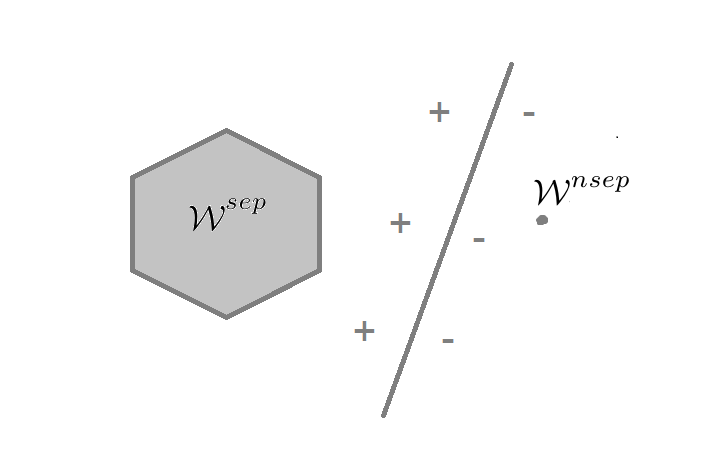
\includegraphics[width=0.8\textwidth]{obrazki/hip}
\caption{Każde dwa rozłączne zbiory wypukłe (geometrycznie figury) można rozdzielic hiperpłaszcz ze względu na pewien iloczyn skalarny, tak że elementy jednego zbioru będą przyjmowały dodatnie wartości iloczynu skalarnego z elementem przestrzeni wektorowej charakteryzującym hiperpłaszczyznę, zaś elementy drugiego ujemne. Jako, że zbiór separowalnych macierzy procesu jest wypukły z definicji i każdy zbiór jednoelementowy jest zbiorem wypukłym, pozwala to dla każdego procesu poszukiwać hiperpłaszczyzn oddzielających ten konkretny proces od zbioru procesów separowalnych. Taką hiperpłaszczyznę nazywa się świadkiem przyczynowości.
}
\label{fig:hip}
\end{figure}
Twierdzenia o separującej hiperpłaszczyźnie mówi, że dla każdych dwóch wypukłych zbiorów albo ich przecięcie nie jest zbiorem pustym, albo istnieje taka hiperpłaszczyzna, że zbiory leżą po obu jej stronach, nierygorystycznie mówiąc. Można to łatwo sobie zobrazować geometrycznie patrząc na rysunek \ref{fig:hip}. Korzystając z tego twierdzenia i faktu, że macierzy separowalnych jest wypukły i zamknięty dla każdego nieseparowalnego procesu $W^{nsep}$, to można stwierdzić, że istnieje taki świadek przyczynowości, że 
\begin{equation}
\Trs \left[ S_{W^{nsep}} W^{nsep} \right] < 0.
\end{equation}
\subsection{Sformułowanie macierzy procesu niezależne od bazy}
Przed dalszym charakteryzowaniem świadków przyczynowości wygodnie jest wprowadzić niezależne od wyboru bazy sformułowanie macierzy procesu.
\begin{definicja}
Operator ${}_XW$ zdefiniowany jest następująco:
\begin{equation}
{}_X W = \frac{\I^X}{d_X} \otimes \Trs_X W.
\end{equation}
\end{definicja}
Operacja ${}_XW$ opisuje operacje wzięcia śladu i zastąpienia tego systemu znormalizowaną macierzą jednostkową.
Warunki na macierz procesu wprowadzone w rozdziale \ref{macierz_procesu} są równoważne z następującymi
\begin{gather}
W \geq 0 \\
\Trs W = d_O \\
W = L_V\left(W\right),
\end{gather}
gdzie $d_0 = d_{A_2} d_{B_2} \dots$ jest iloczynem wymiaru wszystkich systemów wyjściowych, a $L_V$ jest projektorem, zdefiniowanym w \cite{causal_witness}, na pewną podprzestrzeń 
$\mathcal{L_V} \subset \Hx{A_1} \otimes \Hx{A_2} \otimes \Hx{B_1} \otimes \Hx{B_2} \dots$.
W sposób jawny projektor dla przypadku dwustronnego $L_V$ wyraża się następująco:
\begin{equation}
\label{eq:projec2}
L_V(W) = {}_{A_2}W + {}_{B_2}W - {}_{A_2B_2}W - {}_{B_1B_2}W + {}_{A_2B_1B_2}W - {}_{A_1A_2}W + {}_{A_1A_2B_2}W.
\end{equation}
Warto tutaj porównać powyższe równanie do poprzedniego sformułowania macierzy procesu. Zauważa się, że w przypadku wybranej bazy Hilberta-Schmidta
operacja
\begin{equation}
{}_X\left[\sigma_\mu^X \otimes \sigma_\nu^Y\right] = \delta_{\mu0}.
\end{equation}
Należy przypomnieć, że $\sigma_0 = \I$.
Wynika to oczywiście z faktu, że reszta wyrazów jest bezśladowa i $\frac{\Trs \I^X}{d_X} = 1$. Co daje następującą interpretację dla wyrazów występujących w \eqref{eq:projec2}: są to wyrazy zakazane w tym formalizmie, lub bardziej precyzyjnie dany projektor implikuje układ równań liniowych narzucających warunki na współczynniki występujące przy danych macierzach bazowych. Zważywszy na fakt, że jawna postać projektora dla n stron została wyprowadzona w oryginalnym artykule, łatwym zadaniem jest wyprowadzenie warunków na współczynniki przy owych bazach. 
Dla oswojenia się z powyższym projektorem można sprawdzić spełnianie $W = L_V(W)$ przez macierz procesu wprowadzoną w poprzednim rozdziale:
\begin{gather}
W = \frac{1}{4}\left[
\I\I\I\I + \frac{1}{\sqrt{2}}(\I\Z\Z\I + q\Z\I\X\Z + \frac{(1-q)}{2}\Z\I\X\I)
\right],~ 0 \leq q \leq 1. \\ 
\begin{split}
{}_{A_2} W =  \frac{1}{4}\left[
\I\I\I\I + \frac{1}{\sqrt{2}}(q\Z\I\X\Z + \frac{(1-q)}{2}\Z\I\X\I)
\right]
\end{split} \\
{}_{B_2}W =  \frac{1}{4}\left[
\I\I\I\I + \frac{1}{\sqrt{2}}(\I\Z\Z\I + \frac{(1-q)}{2}\Z\I\X\I)
\right] \\
{}_{A_2B_2}W = 
 \frac{1}{4}\left[
\I\I\I\I + \frac{1}{\sqrt{2}}\frac{(1-q)}{2}\Z\I\X\I
\right] \\
{}_{B_1B_2}W =  \frac{1}{4}\left[
\I\I\I\I
\right]\\
{}_{A_2B_1B_2}W =  \frac{1}{4}\left[
\I\I\I\I
\right]\\
{}_{A_1A_2}W =  \frac{1}{4}\left[
\I\I\I\I
\right]\\
{}_{A_1A_2B_2}W =  \frac{1}{4}\left[
\I\I\I\I
\right] \\
W = L_V(W).
\end{gather} W poprzednich obliczeniach korzystano z faktu, że wyłącznie $\I$ jest elementem bazy Hilberta-Schmidta o niezerowym śladzie, konsekwencją tego jest to, że operator ${}_X$ działający na macierz jednostkową na danej pozycji dokonuje trywialnej zmiany, zaś w przeciwnym wypadku usuwa dany wyraz. 
Dowód faktu, że operator $L_V$ rzeczywiście jest projektorem przebiega następująco: operator $L_V$ jest samosprzeżony w sensie iloczynu skalarnego Hilberta-Schmidta
\begin{gather}
A =\sum_{ij} \alpha_{ij} \sigma_i \otimes \sigma_j ,~A \in X \otimes Y \\
B =\sum_{kl} \beta_{kl} \sigma_k \otimes \sigma_l,~B\in X\otimes Y\\
\begin{split}
\langle {}_X A, B \rangle &= \Trs \left[ {}_X A, B\right] = \sum_{ijkl} \Trs\left[ {}_X (\alpha_{ij} \sigma_i \otimes \sigma_j) (\beta_{kl} \sigma_k \otimes \sigma_l)\right] \\
&= \sum_{jkl} \Trs \left[ (\alpha_{0j} \I \otimes \sigma_j) (\beta_{kl} \sigma_k \otimes \sigma_l) \right] = \sum_{jkl} \alpha_{0j} \beta{kl} \Trs \left[ \I \sigma_k\right] \Trs \left[ \sigma_j \sigma_l\right] \\
&= \sum_{jl} \alpha_{0j} \beta_{0l}C \Trs \left[ \sigma_j \sigma_l \right] \\
\langle A, {}_X B \rangle &=  \Trs\left[ (\alpha_{ij} \sigma_i \otimes \sigma_j) ( {}_X \beta_{kl} \sigma_k \otimes \sigma_l)\right] = \sum_{ijl} \Trs \left[ (\alpha_{ij} \I \otimes \sigma_j) (\beta_{0l} \sigma_k \otimes \sigma_l) \right] \\
&= \sum_{jl} \alpha_{0j} \beta_{0l}C \Trs \left[ \sigma_j \sigma_l \right] = \langle {}_X A, B \rangle,
\end{split}
\end{gather} macierze $\{ \sigma_i \}$ tworzą bazę Hilberta-Schmidta, zaś stała C jest związana z stała, do której znormalizowana jest baza. Korzystając z liniowości pokazuje się hermitowskość dla projektora $L_V$. $L_V^2 = L_V$ wykazuje się następująco:
\begin{gather}
\begin{split}
L_V^2(W) &= \left({}_{A_2} + {}_{B_2} - {}_{A_2B_2} - {}_{B_1B_2} + {}_{A_2B_1B_2}- {}_{A_1A_2} + {}_{A_1A_2B_2} \right)\\&\quad\left( {}_{A_2} + {}_{B_2} - {}_{A_2B_2} - {}_{B_1B_2} + {}_{A_2B_1B_2} - {}_{A_1A_2} + {}_{A_1A_2B_2}\right)W
\end{split} \\
\begin{split}
{}_{A_2} L_V(W) &= ({}_{A_2} + {}_{A_2B_2} - {}_{A_2B_2} - {}_{A_2B_1B_2} + {}_{A_2B_1B_2} - {}_{A_1A_2} + {}_{A_1A_2B_2})W \\
&= ({}_{A_2} - {}_{A_1A_2} + {}_{A_1A_2B_2})W
\end{split} \\
{}_{B_2} L_V(W) = ({}_{B_2} - {}_{B_1B_2} + {}_{B_1B_2A_2})W \hspace{5cm}\\
\begin{split}
-{}_{A_2B_2}L_V(W) &= (-{}_{A_2B_2} - {}_{A_2B_2} + {}_{A_2B_2} + {}_{A_2B_1B_2} - {}_{A_2B_1B_2} + {}_{A_1A_2B_2} - {}_{A_1B_1B_2})W \\
&= -{}_{A_2B_2}W
\end{split} \\
\begin{split}
-{}_{B_1B_2}L_V(W) &= (-{}_{A_2B_1B_2} - {}_{B_1B_2} +{}_{A_2B_1B_2} + {}_{B_1B_2} - {}_{A_2B_1B_2} + {}_{A_1A_2B_1B_2} - {}_{A_1A_2B_1B_2})W \\
&= -{}_{A_2B_1B_2}W
\end{split} \\
-{}_{A_1A_2} L_V(W) =-{}_{B_2A_1A_2}W \hspace{5cm}\\
\begin{split}
{}_{A_2B_1B_2}L_V(W) &= ({}_{A_2B_1B_2} + {}_{A_2B_1B_2} -{}_{A_2B_1B_2} - {}_{A_2B_1B_2} + {}_{A_2B_1B_2} - {}_{A_1A_2B_1B_2} + {}_{A_1A_2B_1B_2})W \\
&= {}_{A_2B_1B_2}W
\end{split} \\
{}_{A_1A_2B_2}L_V(W) = {}_{A_1A_2B_2}W \hspace{5cm}\\
\begin{split}
L_V^2(W) =&  ({}_{A_2} - {}_{A_1A_2} + {}_{A_1A_2B_2})W +  ({}_{B_2} - {}_{B_1B_2} + {}_{B_1B_2A_2})W  -{}_{A_2B_2}W - \\
&-{}_{A_2B_1B_2}W  -{}_{B_2A_1A_2}W + {}_{A_2B_1B_2}W + {}_{A_1A_2B_2}W = L_V(W).
\end{split}
\end{gather}
Powyżej korzystano z własności ${}_{XY} = {}_{YX}$, ${}_{XX} = {}_X$ i z faktu, że operator $L_V$ jest symetryczny ze względu na zamianę systemu $A$ i $B$.
\subsection{Poszukiwanie świadka przyczynowości}
Zauważa się, że warunek \eqref{eq:witness_gez} jest równoważny z następującymi dwoma
\begin{gather}
\label{eq:css2}
\Trs \left[ W^{A \prec B} S\right] \geq 0 \\
\label{eq:css}
\Trs \left[ W^{B \prec A} S\right] \geq 0.
\end{gather}
Oczywiście powyższe równania wynikają z definicji stanów separowalnych, jako kombinacji wypukłej macierzy o określonej przyczynowości i liniowości śladu.
Łatwo można zaobserwować, że pozbywając się wyrazów zawierających wyrazy typu $\dots B_2$ usuwamy korelacje wyjścia Boba z pomiarami Alicji co
implikuje, że $A \prec B$. Piszę się, że:
\begin{equation}
{}_{B_2} W = W^{A \prec B},
\end{equation}
lub analogicznie
\begin{equation}
{}_{A_2} W = W^{B \prec A}.
\end{equation}
Wykorzystując powyższą zależność, równanie \eqref{eq:css} możemy zapisać następująco:
\begin{equation}
\Trs \left[ {}_{A_2} W S\right] \geq 0
\end{equation}
Traktując ślad jako iloczyn skalarny $\langle M S \rangle = \Trs MS$ oraz zauważając, że ${}_X$ jest operatorem samosprzężonym równoważne z powyższym
równaniem jest:
\begin{equation}
\Trs \left[ W {}_{A_2}S \right] \geq 0.
\end{equation}
Dla prawidłowych macierzy procesu wystarczającym dla $S$ do bycia świadkiem przyczynowości jest 
\begin{gather}
{}_{A_2} S \geq 0 \\
{}_{B_2} S \geq 0.
\end{gather}
Zauważa się dodatkowo dowolność dodania dowolnego elementu $S^\bot$ z przestrzeni ortogonalnej do $\mathcal{L_V}$, który nie zmieni wartości \ref{eq:witness_gez}, a mianowicie
\begin{equation}
\Trs\left[W\left(S + S^\bot\right)\right] = \Trs\left[WS\right]
\end{equation}
Okazuje się, że powyższe warunki charakteryzują wszystkich świadków przyczynowości.
Co zbierając razem daje:
\begin{tw}
Macierz herimitowska S jest świadkiem przyczynowości wtedy i tylko wtedy, gdy podlega poniższej dekompozycji
\begin{gather}
S = S_P + S^\bot,
\end{gather}
gdzie $S_P$ i $S^\bot$ są takimi macierzami hermitowskimi, że
\begin{gather}
{}_{A_2} S_P \geq 0, {}_{B_2} S_P \geq 0, L_V(S^\bot) = 0.
\end{gather}
\end{tw}
Pokazuje się, że zbiór tak zdefiniowanych świadków przyczynowości jest domkniętym stożkiem wypukłym. Można jednak ograniczyć się z $S$ do przestrzeni 
$\mathcal{L_V}$. Wybierając $S^\bot = L_V(S_P) - S_P$, który może być dowolny. Mamy $L_V(S) = S$. Okazuje się, że taki ograniczony zbiór świadków przyczynowości: $\mathcal{S_V} = \mathcal{S} \cap \mathcal{L_V}$, również jest domkniętym wypukłym stożkiem. Jako, że wybrane elementy ortogonalne do
$\mathcal{L_V}$ nie zmieniają wartości $\Trs WS$, nie zmieniają one też dlatego zdolności S do wykrywania separowalności. 
Dostając pewną macierz $W$ i chcąc zbadać, czy jest ona separowalna, można spróbować znaleźć minimalna wartość $\Trs WS$. W przypadku możliwości 
znalezienia minimum globalnego takiego wyrażenia widzimy, że jeżeli nie uda nam się znaleźć takiego S, że $\Trs WS < 0$ oznacza to, że nie istnieje
taka hiperpłaszczyzna oddzielająca procesy separowalne, więc ten proces też jest separowalny. W przeciwnym wypadku proces jest nieseparowalny.
W celu ograniczenia od dołu skończoną wartością, by możliwe było rozwiązanie problemu numerycznie, na $\Trs SW$ należy narzucić pewien dowolny warunek normujący.
Autorzy oryginalnego artykułu proponują następujący:
\begin{equation}
\Trs \Omega S \leq 1,
\end{equation}
gdzie $\Omega$ jest znormalizowaną macierzą procesu.
Rozpisując powyższą formułę otrzymuje się
\begin{equation}
\Trs\left[ \frac{\Omega \Trs \left[ \Omega \right]}{d_O}S\right]\leq1 \iff \Trs \Omega S \leq \frac{\Trs \Omega}{d_O}
\end{equation}
Ostateczna postać powyżej nierówności pozwala porzucić warunek, by $\Omega$ była znormalizowana co umożliwia przenieść problem optymalizacyjny na stożek wypukły nieznormalizowanych macierzy procesu.
Co można przepisać, jako 
\begin{equation}
\Trs \left[ \Omega(\frac{\I}{d_O} -S) \right] \geq 0
\end{equation}
Łatwo zauważyć, że powyższy warunek jest warunkiem, który muszą spełniać operatory $\frac{\I}{d_O} - S,$ by należały do stożka dualnego macierzy procesu, czyli takiego, że ich iloczyn skalarny jest nieujemny z macierzami procesu.
\begin{definicja}
Optymalnym świadkiem przyczynowości nazywa się optimum globalne poniższego zadania optymalizacyjnego:
\begin{gather}
\min \Trs \left[ WS \right]\\
\text{tak, aby } S \in \mathcal{S_V},~ \frac{\I}{d_O} - S \in \mathcal{W^*_V},
\end{gather}
gdzie $\mathcal{W^*_V}:=\mathcal{W^*} \cap \mathcal{L_V}.~ \mathcal{W^*}$ jest wcześniej wspomnianym stożkiem dualnym do macierzy procesu,
zaś człon $\mathcal{L_V}$ wynika z wcześniej narzuconego warunku na $S \in \mathcal{L_V}$. 
\end{definicja}
Optymalny świadek przyczynowości pozwala stwierdzić, czy dany proces jest separowalny przyczynowo.
Problem ten okazuje się być prawidłowym problemem
programowania liniowego po stożku (\textit{semidefinite programming}, SDP), którego numeryczne rozwiązanie jest zbieżne do optimum globalnego.
Wynika z tego, że rozwiązanie takiego problemu optymalizacyjnego daje kryterium separowalności przyczynowej, z którego można efektywnie korzystać.
\begin{definicja}
Uogólnioną wytrzymałością(\textit{generalized robustness}) nazywa się wartość:
\begin{equation}
R_g(W) = -\Trs\left[ S^*W\right],
\end{equation} gdzie $S^*$ jest optymalnym świadkiem przyczynowości dla macierzy W. Wartość ta odpowiada rozwiązaniu dualnego problemu do problemu optymalnego świadka:
\begin{equation}
\frac{1}{1 + \lambda}\left( W + \lambda\widetilde{\Omega}\right),
\end{equation} ze względu na zmienną $\lambda$
zoptymalizowanej po wszystkich znormalizowanych macierzach procesu $\widetilde{\Omega}$. 
\end{definicja}
Wartość ta określa odporność danego procesu do pozostania nieseparowalnym podczas mieszania z "najgorszym" możliwym szumem. Jest to miara nieseparowalności spełniająca standardowe wymagania, a mianowicie
\begin{description}
\item[Dyskryminacja] $R_g(W) \geq 0$ dla każdej macierzy procesu, przyjmuje wartość 0 wyłącznie dla procesów należących do $\mathcal{W}^{sep}$. 
\item[Wypukłość] $R_g(\sum_i p_i W_i) \leq \sum_i p_i R_g(W_i)$ dla dowolnych macierzy procesu i $p_i \geq 0$ takich, że $\sum_i p_i = 1$. 
\item[Monotoniczność ze względu na lokalne operacje] $R_g\left(\$(W)\right) \leq R_g\left(W\right)$, gdzie $\$(W)$ jest dowolnym procesem, który można 
otrzymać przez złożenie go z lokalnymi odwzorowaniami CPTP.
\end{description}
Można wprowadzić również problem, w którym poszukuje się minimalnej ilości białego szumu potrzebnego do spowodowania, by proces stał się separowalnym. Biały szum może się okazać bardziej adekwatnym modelem szumu niż przypadek pesymistyczny.
\begin{definicja}
Losową wytrzymałością (\textit{random robustness}) nazywa się wielkość:
\begin{equation}
R_r(W) = -\Trs\left[S^* W\right],
\end{equation}
gdzie $S^*$ jest optymalnym rozwiązaniem następującego problemu optymalizacyjnego
\begin{gather}
\min \Trs \left[ WS \right]\\
\text{tak, by } S \in \mathcal{S_V}, \Trs\left[\IO S\right] \leq 1.
\end{gather}
\end{definicja}
W przeciwieństwie do uogólnionej wytrzymałości nie jest to miara nieseparowalności, w sensie poprzednio przytoczonych postulatów, jako że nie jest monotoniczna pod działaniem lokalnych odwzorowań CPTP.
\subsection{Implementacja świadka przyczynowości}
Korzystając chociażby z twierdzenia spektralnego wiadomym jest, że macierz hermitowską S można zapisać jako kombinację liniową następującej postaci
\begin{equation}
S = \sum_{i,j} \gamma_{i,j} \sigma^{A_1A_2}_i \otimes \sigma^{B_1B_2}_j,
\end{equation} gdzie macierze $\sigma \geq 0$. Dodatkowo w $\gamma_{i,j}$ można dodać stałą skalującą tak, aby $\Trs_{A_2} \sigma_i \leq \I^{A_1}$, $\Trs_{B_2} \sigma_j \leq \I^{B_1}$.
Co więcej można dodać do $S$ macierz $\sigma_0^{A_1A_2} \otimes \sigma_0^{B_1B_2}$ o zerowej stałej, która nie zmienia wartości S, tak aby $\sum_i \Trs_{A_2} \sigma^{A_1A_2}_i = \I^{A_1}$ i analogicznie dla strony Boba. Wtedy można traktować macierze $\sigma^{A_1A_2}_i,~ \sigma^{B_1B_2}_j$ jako reprezentacje CJ pewnego instrumentu kwantowego, więc wielkość
\begin{equation}
\Trs \left[ W S \right] = \sum_{i,j} \gamma_{i,j} \Trs\left[ W \sigma^{A_1A_2} \otimes \sigma^{B_1B_2} \right],
\end{equation} gdzie wartość po prawej stronie równania jest oczywiście prawdopodobieństwem zaobserwowania danych odwzorowań, wielkość tę można oszacować eksperymentalnie.
Warto również przypomnieć, że do $S$ można dodać dowolny element z przestrzeni ortogonalnej do przestrzeni $\mathcal{L_V}$, co nie zmienia wartości oczekiwanej świadka, a może skutkować w łatwiejszego do implementacji fizycznie odwzorowania. 
\section{Postulat puryfikacyjny}
Ważnym aktualnie nierozwiązanym problemem występującym w tym formalizmie jest brak jasnego kryterium, które stwierdzałoby, które procesy są możliwe do zrealizowania fizycznie.
Nie wiadomo, czy łamanie nierówności przyczynowych jest możliwie fizyczne, czy wyłącznie jest matematycznym artefaktem. Jasne jednakże jest, że występowanie nieseparowalności jest fizycznie występującym fenomenem, który został potwierdzony doświadczalnie przy realizacji tzw. 
kwantowego przełącznika (\textit{quantum switch})- zasobu, który nie może złamać przyczynowych nierówności - wykorzystując wcześniej opisanego świadka przyczynowości np. w \cite{experiment}. Może to nasuwać postulat, że fizycznie niemożliwe jest naruszenie tych nierówności. Prawdziwość tego postulatu wciąż stoi pod znakiem zapytania. W \cite{purification} autorzy proponują postulat puryfikacyjny (\textit{purification postulate}). Uznają za konieczne, że każda fundamentalna fizycznie poprawna teoria
musi być odwracalna. Motywują się faktem, że każda znana fundamentalna teoria jest odwracalna - taka intuicja sprawdza się do tej pory.
Warto jeszcze dodać, że we wstępie zostały opisany pomiar rzutujący jako nieodwracalny rodzaj ewolucji, jednakże można modelować pomiar w sposób niewymagający takich pomiarów modelując układ pomiarowy, jako system kwantowy, który ewoluuje unitarnie wraz z mierzonym systemem, co pokazano np. w
\cite{reversible}. 
%W celu dalszego opisu postulatu koniecznym jest opisanie, jak rozumiana jest odwracalność w kontekście procesów. W tym celu procesy są poszerzone o globalną przeszłość i globalną przyszłość. Rozumie się je jako operacje, które odwzorowują stany w globalnej przeszłości do stanów w globalnej przyszłości, które przechodzą przez region o nieokreślonej przyczynowości lokalnych laboratoriów opisywanych właśnie przez te macierze. Co sprowadza do definicji czystych procesów (\textit{pure processes}), jako procesów, które w sposób unitarny transformują przyszłość do przeszłości, gdy w lokalnych laboratoriach zostaną zaaplikowane odpowiednie unitarne transformacje. Ta definicja sprowadza do ich postulatu, który mówi, że procesy są puryfikowalne wtedy i tylko wtedy, gdy da się zaprezentować je jako czyste procesy w większej przestrzeni i tylko takie procesy są implementowalne. Autorzy postulatu dodatkowo zauważają, że
%o ile żaden znany dwustronny proces łamiący nierówności przyczynowe nie okazał się być puryfikowalnym, to istnieje proces trzystronny, który jest puryfikowalny i może łamać przyczynowe nierówności, więc jeżeli niemożność łamania przyczynowych nierówności uznałoby się za prawo natury, a ten postulat za prawdziwy, to
%byłby on konieczny, a nie wystarczający. 
\begin{figure}[t]
\centering
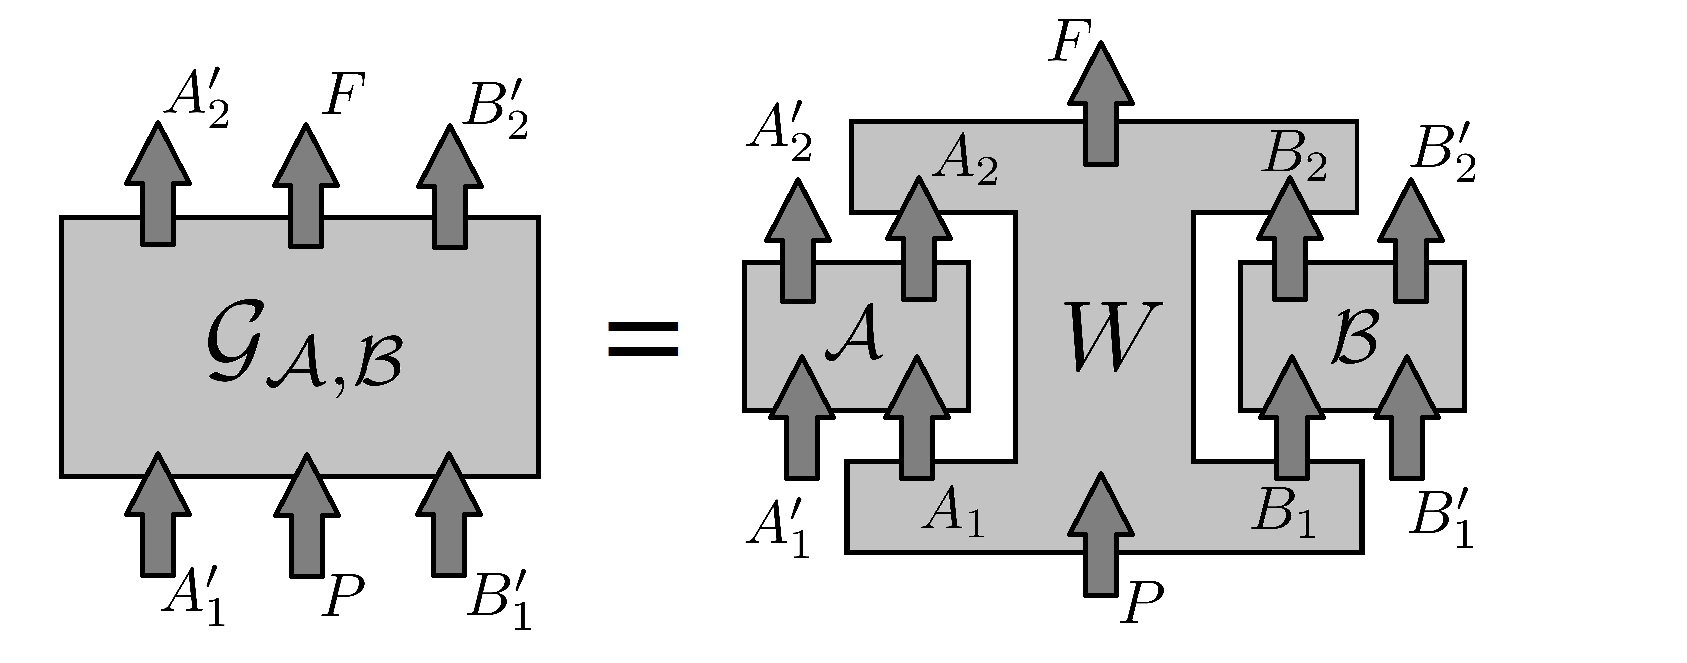
\includegraphics[width=0.6\textwidth]{obrazki/done1}
\caption{
Rysunek symbolizuje działanie procesu $W$ jako funkcje wyższego rzędu odwzorowań $\mathcal{A}$ i $\mathcal{B}$, która dla danych odwzorowań zwraca odwzorowanie 
$\mathcal{G_{A,B}}$ reprezentującą transformację, która przechodzi z globalnej przeszłości do globalnej przyszłości.
}
\label{higherordermap}
\end{figure}
%We wcześniejszych rozdziałach proces był definiowany jako zasób, który definiował wszystkie statystyki pomiarów dla danych instrumentów, lub równoważnie jako funkcja, która transformuje odwzorowania CP do prawdopodobieństw. Wprowadzenie pojęcia puryfikacji wymaga zmiany definicji na biliniową funkcję działająca trywialnie na \textit{ancille}, która odwzoruje
%$\mathcal{A}$ i $\mathcal{B}$ do $\mathcal{G_{A,B}}$, gdzie $\mathcal{A}$ jest odwzorowanie CPTP z $A_1, A'_1$ do $A_2, A'_2$, analogicznie $\mathcal{B}$ jest mapą CPTP z
%$B_1, B'_1$ do $B_2, B'_2$, zaś $\mathcal{G_{A,B}}$ mapą CPTP z $P, A'_1, A'_2$ do $F, B'_1, B'_2$. Primem oznaczono \textit{ancille}. Ponownie przez A niepisane kaligraficznie oznaczać będzie się reprezentacje CJ odpowiednich map, podobnie dla innych map. Taka definicja nie jest w żaden sposób sprzeczna z tymi podanymi wcześniej, gdyż ma ona służyć jedynie jako droga do zbudowania narzędzia stwierdzającego, czy dany proces jest fizyczny bądź nie. Trzeba zaznaczyć, iż w tym rozdziale definicja izomorfizmu CJ jest zmieniona o transpozycję, która wcześniej została wprowadzona ze względu na wygodę, teraz jednakże może sprawiać, że pewne odwzorowania CP 
%mogą zostać mapowane na macierze niedodatnie. Jako że żadna przestrzeń nie może sygnalizować P, a przestrzeń F nie może sygnalizować do żadnej innej,
%można je interpretować odpowiednio jako globalną przeszłość i globalną przyszłość. Oczywiście tak zdefiniowany proces ma swoją reprezentację jako macierz - pisze się
%Macierz procesu (puryfikacyjną) definiuje się jako liniową funkcje wyższego rzędu odwzorowań, która na wejściu przyjmuje odwzorowania opisujące wykonywane przez laboratoria czynności $A$ i $B$, a na wyjściu zwraca odwzorowanie CPTP opisujące przejście systemu z globalnej przeszłości oraz systemów pomocniczych $P, A'_1 B'_1$ do globalnej przyszłości $F, A'_2, B'_2$. Odwzorowanie to otrzymuje się z następującej formuły:
%\begin{equation}
%\label{eq:longnp}
%G_{A,B} = \Trs_{A_1A_2B_1B_2} \left[ W^{T_{A_1A_2B_1B_2}} (A\otimes B)\right],
%\end{equation}
%gdzie $W \in A_1 \otimes A_2 \otimes A'_1 \otimes A'_2 \otimes B_1 \otimes B_2 \otimes B'_1 \otimes B'_2 \otimes F \otimes P$. W powyższym równaniu macierze jednostkowe na \textit{ancillach}, globalnej przyszłości i przeszłości pozostały niejawne.
%Korzystając z definicji macierzy wiadomo, że powyższe równanie opisuję najogólniejsza metodę transformacji liniowych map A i B. Dodatkowo wyjściowe odwzorowanie musi działać trywialnie na systemy pomocnicze. Co więcej puryfikacyjna macierz procesu musi dodatkowo spełniać następujące warunki:
\begin{definicja}
Najogólniejsze liniowe odwzorowanie odwzorowań CPTP $\mathcal{A}: \mathcal{L}(\Hx{A_1} \otimes \Hx{A'_1}) \mapsto  \mathcal{L}(\Hx{A_2} \otimes \Hx{A'_2})$ i $\mathcal{B}: \mathcal{L}(\Hx{B_1} \otimes \Hx{B'_1}) \mapsto  \mathcal{L}(\Hx{B_2} \otimes \Hx{B'_2})$ na odwzorowanie CPTP $\mathcal{G_{A,B}}: \mathcal{L}(\Hx{A'_1} \otimes \Hx{P} \otimes \Hx{B'_1} \mapsto \mathcal{L}(\Hx{A'_2} \otimes \Hx{F} \otimes \Hx{B'_2}$ nazywa się procesem (puryfikacyjnym) $\mathcal{W}: \mathcal{A} \otimes \mathcal{B} \mapsto \mathcal{G_{A,B}}$. Macierzą procesu nazywa się macierz CJ procesu, która otrzymuje się z formuły\cite{purification}
\begin{equation}
G_{A,B} = \Trs_{A_1A_2B_1B_2}\left[ \I^{A'_1B'_1A'_2B'_2} \otimes {W^{PA_1A_2B_1B_2F}}^{T_{A_1A_2B_1B_2}} \left( \I^{PF} \otimes A^T \otimes B^T\right)\right],
\end{equation}
gdzie $A = \MCJ({\mathcal{A}})$, $B = \MCJ(\mathcal{B})$, $G_{A,B} = \MCJ(\mathcal{G_{A,B}})$.
Macierz procesu musi spełniać następujące warunki:
\begin{gather}
W \geq 0 \\
\Trs W = d_{A_2}d_{B_2}d_P \\
W = L_V(W).
\end{gather} 
\end{definicja}
Jawna postać powyższego projektora jest następująca:
\begin{align}
\begin{split}
L_V(W) =& W -{}_FW + {}_{A_2F}W + {}_{B_2}W - {}_{A_2B_2F}W\\ &- {}_{A_1A_2F}W + {}_{A_1A_2B_2F}W - {}_{B_1B_2F}W \\&+ {}_{A_2B_1B_2F}W - {}_{A_1A_2B_1B_2F}W + {}_{PA_1A_2B_1B_2F}W.
\end{split}
\end{align}
Ważnym spostrzeżeniem jest fakt, który przekonuje do słuszności poprzedniej definicji macierzy procesu, definiując $W' = {}_{PF}W$ i korzystając z faktu, że
${}_{XX}W = {}_{X}W$, po elementarnych przekształceniach otrzymuje się, że
\begin{equation}
L_V(W') = {}_{A_2}W' + {}_{B_2}W' - {}_{A_2B_2}W' - {}_{B_1B_2}W' + {}_{A_2B_1B_2}W' - {}_{A_1A_2}W' + {}_{A_1A_2B_2}W'.
\end{equation}
Powyższy projektor ma takie same wyrazy, jak ten zdefiniowany w \eqref{eq:projec2}.
Każdy dwustronny proces zdefiniowany w poprzednim sensie rozszerzony o odpowiednio znormalizowaną jednostkową przyszłość i przeszłość spełnia warunki narzucone powyżej, co pokazuje, że każdy proces dwustronny, definiowany jak poprzednio, jest zgodny z tą definicją.
Rówanie \eqref{eq:longnp} może być skrócone z wykorzystaniem iloczynu łączącego(\textit{link product}).
W celu zapisania postaci CJ złożenia pewnych dwóch funkcji można obliczyć jawną postać CJ $\MCJ(\mathcal{M} \circ \mathcal{N})$. Wygodniejszym
jednak często okazuje się być wcześniej wspomniany iloczyn łączący. 
\begin{definicja}
Iloczyn łączący dwóch macierzy definiowany jest jako
\begin{equation}
N * M = \Trs_{I\cap J}\left[ (\I^{J\setminus I} \otimes M^{T_{I\cap J}})(N \otimes \I^{I\setminus J})\right],
\end{equation}
gdzie $M \in \bigotimes_{i \in I} A^i,~N \in \bigotimes_{j \in J} A^j$.
\end{definicja} W skrajnych przypadkach gdy $I \cap J = \emptyset$, $N*M$ to po prostu $N \otimes M$, a
gdy $I \cap J = I = J$ to $N * M = \Trs M^T N$. Ułatwić zrozumienie iloczynu łączącego w przypadkach bardziej skomplikowanych pozwala następujący przykład:
\begin{equation}
\begin{split}
\I\X\Y^{ABC} * \Y\Y\Z^{BCD} &= \Trs_{BC} \left[ \left(\I^{A} \otimes {\Y\Y\Z^{BCD}}^{T_{BC}}\right)\left(\I\X\Y^{ABC} \otimes \I^D\right)\right] \\
&= \Trs_{BC} \left[ \I^A \otimes (-\Y\X)^{B} \otimes {-\Y\Y}^{C} \otimes \Z^{D}\right] \\
&= \I^{A} \otimes \Z^{D} \Trs_{B} \left[ -\Y\X \right]\Trs_{C}\left[-\Y\Y\right] \\
&= \I^{A} \otimes \Z^{D} 0 \cdot (-1) \\
&= 0
\end{split}
\end{equation}
Znając iloczyn łączący w sposób bardzo elegancki można zapisać dwustronny proces jako
\begin{equation}
G_{A,B} = W * (A \otimes B).
\end{equation}
\subsection{Czysty proces}
\begin{definicja}
Czysty proces definiuje się taki proces, dla którego istnieje taka transformacja unitarna $U_W$, że można zapisać proces ten jako
\begin{equation}
W_{czysty} = \KKet{U_W}\BBra{U_W}.
\end{equation}
\end{definicja}
Faktem jest, że czysty proces odwzorowuje unitarne odwzorowania $A$ i $B$ na macierz unitarną. Szkic dowodu przebiega następująco,
wybierając $\mathcal{A}$, $\mathcal{B}$, jako operacje $\bf{SWAP}$ (rysunek \ref{swap}), które odpowiednio zamieniają \textit{ancille} z oryginalnymi systemami. Metodę obliczenia wektora CJ operacji $\bf{SWAP}$ przytoczono poniżej:
\begin{equation}
\begin{split}
\KKet{\bf{SWAP}} &= \sum_i \Ket{i}^{A_1A'_1} \otimes \textbf{SWAP} \Ket{i}^{A_1A'_1} = \sum_{ij} \Ket{i}^{A_1}\Ket{j}^{A'_1} \otimes \textbf{SWAP} \Ket{i}^{A_2}\Ket{j}^{A'_2} \\&= \sum_{ij} \Ket{i}\Ket{i}^{A_1A'_2} \otimes \Ket{j}\Ket{j}^{A'_1A_2} 
= \KKet{\I}^{A_1A'_2}\KKet{\I}^{A'_1A_2}.
\end{split}
\end{equation}
\begin{figure}[t]
\centering
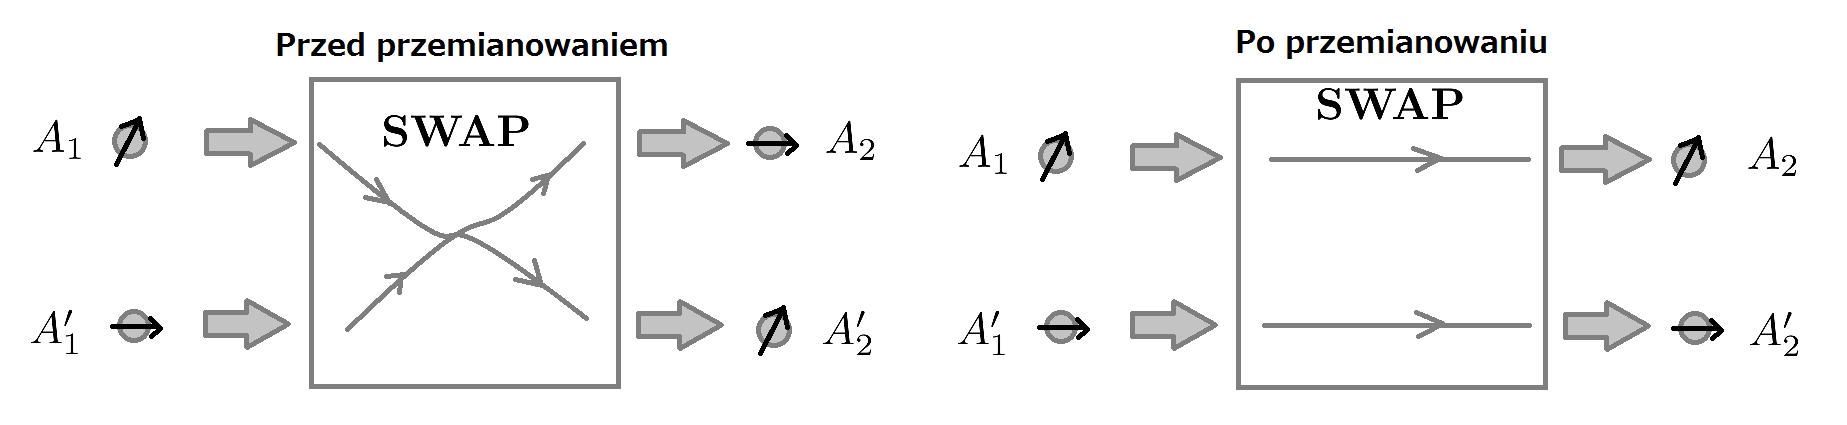
\includegraphics[width=0.95\textwidth]{obrazki/swap}
\caption{Rysunek schematycznie przedstawia działanie operacji $\bf{SWAP}$. Na wejściu Alicja otrzymuje system złożony np. w stanie $\rho^{A_1} \otimes \rho'^{A'_1}$ następnie aplikuje unitarną macierz $\bf{SWAP}$ definiowaną następująco $\textbf{SWAP} = \sum_{ij} \Ket{ij}\Bra{ji}$, a na wyjściu otrzymuje system w stanie $\rho'^{A_2} \otimes \rho^{A'_2}$. Postać CJ tej macierzy to: $\KKet{\I}\BBra{\I}^{A_1A'_2} \otimes \KKet{\I}\BBra{\I}^{A'_1A_2}$.Warto również zauważyć, że po przemianowaniu systemów wyjściowych $A_2 \to A'_2$, $A'_2 \to A_2$ operacja $\bf{SWAP}$ działa trywialnie.}
\label{swap}
\end{figure}
Korzystając z powyższego wyniku można zapisać:
\begin{equation}
G_{A,B} = W * \left( \KKet{\I}\BBra{\I}^{A'_1 A_2} \KKet{\I}\BBra{\I}^{A_1A'_2} \otimes \KKet{\I}\BBra{\I}^{B'_1 B_2} \KKet{\I}\BBra{\I}^{B_1B'_2}\right) = W,
\end{equation}
gdzie po prawej stronie równania przemianowano nazwy odpowiednich przestrzeni. Przekształcenie te ilustrują istnienie odwzorowań, które są przekształcane w macierz unitarną. W ogólności:
\begin{gather}
W = \KKet{U_W}\BBra{U_W} \\
A = \KKet{U_A}\BBra{U_A} \\
B = \KKet{U_B}\BBra{U_B}.
\end{gather}
Następnie
\begin{equation}
G_{A,B} = \KKet{U_W}\BBra{U_W} * \left( \KKet{U_A}\BBra{U_A} \otimes \KKet{U_B}\BBra{U_B} \right) = \KKet{U_G}\BBra{U_G},
\end{equation} gdzie 
\begin{equation}
U_G^{A'_1B'_1P} = \Trs_{A_1B_1} \left[ \left( U_W^{PA_1B_1} \otimes \I^{A'_1B'_1}\right) \left( \I^P \otimes U_A^{A_1A_1'} \otimes U_B^{B_1B'_1}\right)\right]
\end{equation}
Z założenia mamy, że $\mathcal{G_{A,B}}$ jest CPTP, więc $\Trs_{A'_2B'_2F} G_{A,B} = \I^{A'_1B'_1P}$. Podstawiając tu $\KKet{U_G}\BBra{U_G}$ dostaje się
\begin{equation}
\Trs_{A'_2B'_2F} \KKet{U_G}\BBra{U_G} = U^\dag_G U_G = \I^{A'_1B'_1P},
\end{equation}
co kończy dowód.
\subsection{Proces puryfikowalny}
\begin{definicja}
Proces puryfikowalny $W$ definiuje się jako proces dla, którego można znaleźć proces czysty $S$ spełniający następującą równość:
\begin{equation}
\label{eq:purif}
W^{A_1A_2A'_1A'_2B_1B_2B'_1B'_2} = S^{A_1A_2A'_1A'_2B_1B_2B'_1B'_2PF} * \left( \Ket{0}\Bra{0}^P \otimes \I^F \right),
\end{equation}
\end{definicja}
Definicja ta jest zgodna tylko z tymi macierzami procesu, które można odzyskać z procesu czystego, gdy w globalnej przeszłości umieści się ustalony stan i wykona się ślad częściowy po globalnej przeszłości. Odpowiada to sytuacji, w której nie obserwuje się globalnej przeszłości i przyszłości.
Postuluje się, że wyłącznie procesy czyste można skonstruować fizycznie, gdyby było inaczej zachwiana byłaby zasada odwracalności, która jest uznawana za kluczową.
\subsection{Warunki konieczne i wystarczające}
\begin{tw}
Proces jest czysty wtedy i tylko wtedy, gdy spełnia poniższe warunki
\begin{equation}
\begin{gathered}
\forall i,j ~L^\perp_V\left(\Ket{w_i}\Bra{w_j}\right) = 0 \\
\Bra{w_i}\Ket{w_j} = d_{A_2}d_{B_2}\delta{ij} \\
L^\perp_V = \I - L_V  \\
\Ket{w_\psi} := \Bra{\psi^*}^P \KKet{U_S}.
\end{gathered}
\end{equation} 
\end{tw}
W celu wyprowadzenia powyższych zależności na początku zauważa się, że:
\begin{equation}
\KKet{U_S} \BBra{U_S} * (\Ket{\psi}\Bra{\psi}^P \otimes \I^F) = \Ket{w_\psi} \Bra{w_\psi} * 1^F = \Trs_F \Ket{w_\psi} \Bra{w_\psi}
\end{equation}
Równanie \eqref{eq:purif} zapisuje się
\begin{equation}
\label{eq:trpurif}
W = \Trs_F \Ket{w_0}\Bra{w_0},
\end{equation}
gdzie $\Ket{w_0}$ oznacza $\Bra{0}^P\KKet{U_S}$.
Wcześniej narzucano, by S mapowało A i B na inną prawidłowe odwzorowanie CPTP.
Ten warunek można zreformułować w jawny sposób przy pomocy stanów $\Ket{\psi}$.
S jest prawidłowym procesem, kiedy $[ S * (A \otimes B)] * \Ket{\psi}\Bra{\psi}^P$ jest prawidłowym stanem kwantowym. Wynika to z faktu, że narzucony został warunek na macierz procesu, by przekształcała odwzorowania $A$ i $B$ na prawidłowe odwzorowania CPTP, które przekształcają każdy poprawny stan na inny poprawny stan. Wychodząc z drugiej strony można wywnioskować, że jeżeli wynik zadziałania macierzą procesu na odwzorowaniach przekształca wszystkie poprawne stany na inne poprawne stany to musi być to prawidłowy wynik.
Ważnym jednakże jest zauważyć, że
\begin{equation}
[S * (A \otimes B)] * \Ket{\psi}\Bra{\psi} = (S * \KP \BP^P) * (A \otimes B).
\end{equation}
Warunek, by prawa strona równania produkowała prawidłowe stany dla każdego stanu i każdych dwóch odwzorowań jest równoważny z warunkiem, by proces z trywialną przeszłością $(S*\Ket{\psi}\Bra{\psi}^P$ produkował prawidłowe odwzorowania CPTP z trywialną przeszłością z prawidłowych odwzorowań CPTP.
Zapisując jawnie ten warunek otrzymuje się
\begin{gather}
\forall \Ket{\psi} ~(S * \KP \BP) = \Ket{w_\psi}\Bra{w_\psi} = L_V(\Ket{w_\psi}\Bra{w_\psi}) \nonumber \\
\label{eq:purifproj}
 \Trs \Ket{w_\psi} \Bra{w_\psi} = d_{A_2}d_{B_2},
\end{gather}
gdzie $L_V$ jest poprzednio zdefiniowanym projektorem z $d_P$ = 1.
Równanie \eqref{eq:trpurif} można zidentyfikować jako standardową puryfikację stanów mieszanych w przestrzeni mniej wymiarowej jako stanów
czystych w przestrzeniach więcej wymiarowych. Dla macierzy o rozkładzie spektralnym danym
\begin{equation}
W = \sum^{r-1}_i \lambda_i \Ket{\lambda_i}\Bra{\lambda_i},
\end{equation}
gdzie $\lambda_i$ to niezerowe wartości własne, a $\Ket{\lambda_i}$ to odpowiadające im wektory własne.
Poprawną puryfikacją dla takiej macierzy jest
\begin{equation}
\Ket{w_0} = \sum^{r-1}_i \sqrt{\lambda_i} \Ket{\lambda_i} \Ket{i},
\end{equation}
co można łatwo sprawdzić. Puryfikacja ta jest unikatowa z dokładnością do pewnej izometrii V na puryfikowanym systemie, lecz taka izometria nie zmienia
poprawności stanów zwracanych przez proces, więc można ją wybrać jako identyczność bez utraty ogólności, jego przyszłość jako trywialną, więc rozmiar puryfikowanego systemu jako rząd $W$. Pozwala to wybrać $r^2$ wymiarową bazę dla puryfikowanych macierzy. Zapisać wtedy można wektory
$\Ket{w_\psi}$ w tej bazie, jako $\sum^{r-1}_i \alpha_i \Ket{w_i}$. Korzystając teraz z liniowości operacji w warunkach \eqref{eq:purifproj} i cykliczności śladu przepisać je można jako
\begin{gather}
\forall i,j ~L^\perp_V\left(\Ket{w_i}\Bra{w_j}\right) = 0 \nonumber\\
\Bra{w_i}\Ket{w_j} = d_{A_2}d_{B_2}\delta{ij} \\
L^\perp_V = \I - L_V \nonumber,
\end{gather} gdzie $\Ket{w_i} := \Bra{i}^P \KKet{U_S}$.

\subsection{Warunek konieczny}
Okazuje się jednakże, że znalezienie takiego zbioru wektorów $\{ \Ket{v_i} \}$ jest problemem trudnym, gdyż warunek $L^\perp_V(\Ket{v_i}\Bra{v_j})=0$ jest kwadratowy. Dlatego w duchu artykułu, który wprowadził puryfikację 
zostanie tutaj opisany i wyprowadzony warunek konieczny, który jest łatwy do sprawdzenia. Procesy, które nie spełniają tego warunku będą więc niepuryfikowalne, zaś dla reszty będzie niekonkluzywny. Wektor $\Ket{v_0}$ jest ściśle określony dla danej macierzy, jego postać jest znana, więc 
warunek $\LPV(\Ket{v_i}\Bra{v_0}) = 0$ jest liniowy co pozwala scharakteryzować przestrzeń $V_W$ formowaną przez wektory, które je spełniają.
W celu skonstruowania ortonormalnej bazy dla $V_W$ wykorzystuje się $\Pi_\LPV$ zdefiniowany następująco
\begin{equation}
\forall i,j ~\Pi_\LPV \KKet{\Ket{i}\Bra{j}} = \KKet{\LPV(\Ket{i}\Bra{j})}
\end{equation}
Otrzymuje się wtedy, że
\begin{equation}
\LPV(\Ket{v}\Bra{v_0}) = 0 \iff \Pi_\LPV \Ket{v^*_0} \Ket{v} = 0
\end{equation}
Definiując dalej operator $O_W$ dany następująco
\begin{equation}
O_W:= \left(\Bra{w^*_0} \otimes \I\right) \Pi_\LPV \left( \Ket{w^*_0} \otimes \I\right)
\end{equation}
i aplikując go na $\Ket{v}$
\begin{equation}
O_W\Ket{v} = 0 \iff \Pi_\LPV \Ket{w^*_0} \Ket{v} = 0.
\end{equation}
Jeżeli $\Ket{v}$ ma spełniać powyższy warunek, niezerowe składowe może mieć wyłącznie przy tych wektorach bazowych, które odpowiadają wektorom własnym tego operatora, przy których stoją zerowe wartości własne, lub równoważnie wektory własne $O_W$ o zerowych wartościach własnych rozpinają przestrzeń $V_W$. Niech teraz przez $\{ \Ket{r_i}\}$ dane będą właśnie te wektory tworzące ortonormalna bazę w $V_W$ oraz niech $R = \sum_i \Ket{i}\Bra{r_i}$. Ograniczyć można ten projektor do przestrzeni $V^*_W \otimes V_W$ w następujący sposób
\begin{equation}
\Pi_{\LPV|V_W} = \left(R^* \otimes R \right) \Pi_\LPV \left(R^{*\dag} \otimes R^\dag \right)
\end{equation}
Niech teraz $\{ \Ket{m_k} \}^{d_m-1}_{k=0}$ będzie zbiorem wektorów własnych $\Pi_{\LPV|V_W}$ z niezerową wartością własną. Korzystając z argumentu analogicznego do tego powyżej 
\begin{equation}
\Pi_{\LPV|V_W} \Ket{v^*_j}\Ket{v_i} = 0 \iff \forall k \Bra{v^*_j} \Bra{v_i} \Ket{m_k} = 0
\end{equation}
Można teraz spostrzec, że powyższy warunek wygodnie przepisać na
\begin{gather}
\Bra{v^*_j} \Bra{v_i} \Ket{m_k} = \Bra{v_i} M_k \Ket{v_j} \\
\KKet{M_k} = \Ket{m_k}.
\end{gather}
W ogólności macierze $M_k$ nie są hermitowskie, a konieczne są rzeczywiste wartości własne w celu skorzystania z twierdzenia, które zaraz zostanie przytoczone.
Definiuje się
\begin{gather}
C_k = M_k + M^\dag_k
C_{k+d_m} = i(M_k - M_k^\dag)
\end{gather}
Widać oczywiście, że $\frac{C_k-iC_{k+d_m}}{2} = M_k$, a same macierze $C_k$ zostały zdefiniowane jako hermitowskie. Daje to możliwość zapisania, że
\begin{equation}
\Pi_{\LPV|V_W} \Ket{v^*_j}\Ket{v_i} = 0 \iff \forall k \Bra{v_i} C_k \Ket{v_j}
\end{equation}
Dalsze rozwijanie i badanie tego warunku wystarczającego jest otwarty problemem. Udowodniono jednak w opisywanym artykule, że
wymiar przestrzeni, której wektory spełniają
\begin{equation}
\Bra{v'}C_k\Ket{v} = 0
\end{equation} równy jest 
\begin{equation}
d_{C_k} = n_{k0} + \min({n_{k+}, n_{k-}}),
\end{equation} gdzie $n_0, n_k+, n_k-$ są odpowiednio liczbą zerowych, dodatnich i ujemnych wartości własnych k-tej macierzy. Intuicyjne uzasadnienie tego twierdzenia może być następujące: dostępnych jest $n_0$ składowych, które nie wpływają na ten wynik oraz $\min({n_{k+}, n_{k-}})$, które trzeba wyzerować odpowiednio drugim znakiem. Wybierając znak, którego jest więcej, zabrakłoby po prostu składowych do ich wyzerowania.
Toteż prostym ograniczeniem, które okazuje się być w wielu przypadkach nietrywialne jest wzięcie rozmiaru najmniejszej przestrzeni, jeżeli będzie ona mniejsza niż rząd $W$ to macierz będzie niepuryfikowalna, lub zwięźle
\begin{gather}
\text{W jest puryfikowalne} \implies d_{max}(W) \geq \Rank(W) \\
d_{max}(W) := \min_i d_{C_i} 
\end{gather}
\section{Przykłady}
W rozdziale trzecim podano przykład procesu, które może łamać przyczynowe nierówności. Okazuje się, że ten proces nie jest puryfikowalny dla skrajnego $q = 1$, dla $q=0$ jest puryfikowalny, bo przyczynowy, zaś ze względu na złożoność obliczeniową i brak dostępnych wyników w literaturze nie jest wiadome, dla jakich q ten proces jest puryfikowalny.

Kolejnymi interesującymi przykładami są kanały kwantowe. Wektor procesu dla kanału kwantowego jest następujący:
\begin{equation}
\Ket{w_{channel}}^{A \prec B} = \KKet{\I}^{PA_1}\KKet{\I}^{A_2B_1}\KKet{\I}^{B_2F}.
\end{equation}
Reprezentuje on oczywiście zasób, które ma ściśle określoną przyczynowość, dlatego nie może złamać żadnych nierówności przyczynowych.
Biorąc proces następujący
\begin{equation}
a\Ket{w_{channel}}\Bra{w_{channel}}^{A \prec B} + b\Ket{w_{channel}}\Bra{w_{channel}}^{B \prec A},
\end{equation} warunek normujący daje, że $a+b=1$, więc ewidentnie proces jest separowalny. Co za tym idzie on również nie może złamać nierówności przyczynowych. Taki zasób można interpretować jako probabilistyczny kanał, który z pewnym prawdopodobieństwem decyduje, kto jest przed kim.
Eksplorując dalej procesy związane w prosty sposób z kanałami można zadać sobie pytanie, co w takim razie dzieje się z spójnym zmieszanym kanałem, niech wektor procesu będzie dany jako
\begin{equation}
\Ket{w_{procesu}} = a\Ket{w_{channel}}^{A \prec B} + b\Ket{w_{channel}}^{B \prec A}
\end{equation}
Okazuje się jednakże, że niestety proces dany tym wektorem nie należy do przestrzeni poprawnych procesów, gdy dwa współczynniki są różne od zera. W celu uratowania tego wybornego pomysłu spróbowano wziąć 
\begin{equation}
W' = CL_V(W).
\end{equation}
$C$ jest stałą normalizacyjną równą $\frac{d_O}{\Trs W'}$.
W celu prób złamania nierówności danej w trzecim rozdziale wykorzystano następujący protokół. Gdyby dany był idealny dwustronny kanał, można by otrzymać system w jednym laboratorium, zmierzyć $\Ket{i}\Bra{i}$ i powiązać przesyłany bit z odebranym stanem, przypisać odpowiednio swój bit do stanu i wysłać go do drugiego laboratorium. Idąc za pomysłem, że proces powyższy reprezentuje pewnego rodzaju pozostałość z takiego idealnego dwustronnego kanału. przyjmuje się właśnie tę procedurę. Odpowiednie odwzorowania są więc dane
\begin{gather}
\eta(x,a) = \Ket{x}\Bra{x} \otimes \Ket{a}\Bra{a} \\
\xi(y,b,b') = \eta(y,b)
\end{gather}
Pamiętając, że prawdopodobieństwo jest dane jak zwyczaj, czyli
\begin{equation}
\Pr(x,y|a,b,b`) = \Trs\left\{{W\left[\eta(x,a) \otimes \xi(y,b,b') \right]}\right\}
\end{equation}
Okazuje się, że prawdopodobieństwo sukcesu w grze zdefiniowanej w rozdziale trzecim wynosi $0.8$ dla $a=b$, który jest równym połączeniem dwóch kanałów.
Niestety radość musi ukrócić fakt, że powyższa macierz okazuje się nie być nieujemna. Dodając najmniejszą ilość białego szumu takiego, że $W'$ będzie nieujemne, czyli
\begin{equation}
W'' = W' + \lambda_{min} \I,
\end{equation} gdzie $\lambda_{min}$ to najmniejsza wartość własna.
Otrzymuje się prawdopodobieństwo równe około $0.68$, co niestety ujmuje przydatności i wyjątkowości takiego zasobu. Co niestety zmusza do szukania innych ciekawych implementowalnych fizycznie procesów.
W celu spelnienia warunku normalizacyjnego $a + b \leq C$, gdzie C jest pewną stałą, dlatego bez utraty ogólności można wybierać $a + b = 1$ i następnie dokonywać procesu renormalizacji. Na rysunku \ref{fig:bichannel} pokazano prawdopodobieństwo sukcesu dla rodziny procesów generowanych powyżej opisaną metodą.
\begin{figure}[t]
\centering

\includegraphics[width=0.5\textwidth]{obrazki/probchannel.png}
\caption{Wykres pokazujący zależność między a a prawdopodobieństwem sukcesu}
\label{fig:bichannel}
\end{figure}

Bardzo ważnym przykładem, który został zaimplementowany fizycznie, który potwierdza występowanie w fizyce nieprzyczynowego porządku jest kwantowy przełącznik (\textit{quantum switch}). Jest to proces, w którym kanały kwantowe są w superpozycji zależnej od stanów w przeszłości. Jego wektor wygląda następująco
\begin{equation}
\Ket{w_{switch}} = \Ket{0}^{P_1}\KKet{\I}^{P_2A_1}\KKet{\I}^{A_2B_1}\KKet{\I}^{B_2F_2}\Ket{0}^{F_1}+\Ket{1}^{P_1}\KKet{\I}^{P_2B_1}\KKet{\I}^{B_2A_1}\KKet{\I}^{A_2F_2}\Ket{1}^{F_1},
\end{equation} gdzie $F = F_1 \otimes F_2$, $P = P_1 \otimes P_2$. Proces ten jest ewidentnie reprezentacją wektorową CJ pewnego unitarnego operatora. Wystarczy zaobserwować, że działając na proces macierzą unitarną postaci
\begin{equation}
U = \I^{P_1P_2A_1A_2B_1B_2F_1}\otimes\Ket{0}\Bra{0}^{F_2} + \I^{P_1P_2} \otimes \mathbf{SWAP}^{A_1B_1} \otimes \mathbf{SWAP}^{A_2B_2} \otimes \Ket{1}\Bra{1}^{F_2},
\end{equation}
otrzymuje się wektor CJ macierzy jednostkowej. Wynika z tego fakt, że sam proces jest wektorem CJ macierzy unitarnej.
Kubit kontrolny z $P_1$ pozostaje niezmieniony zaś badając zmianę stanu z $P_2$ można dowiedzieć się, jaką "drogę" przebyły. Taki zasób nie jest w stanie złamać żadnych nierówności przyczynowych.
Nie jest żaden znany puryfikowalny przykład w literaturze, który byłby w stanie złamać przyczynowe nierówności, jednakże znany jest proces trzystronny, wprowadzony w \cite{logic}, który jest w stanie złamać przyczynowe nierówności. 
\begin{equation}
W_{det} = \sum_{a,b,c} \Ket{a,b,c}\Bra{a,b,c} \otimes \Ket{\neg b \land c, \neg c\land a \neg a\land b} \Bra{\neg b \land c, \neg c\land a ,\neg a\land b},
\end{equation} systemy zostały zapisane w następującej kolejności $A_2B_2C_2A_1B_1C_1$. Korzystając ze standardowej metody zamieniania nieodwracalnych logicznych funkcji w odwracalne pisze się zamienia się
$\Ket{x} \mapsto \Ket{f(x)}$ na $\Ket{x}\Ket{y} \mapsto \Ket{x}\Ket{y \oplus f(x)}$ wykorzystując to powyższy proces można przepisać w postaci wektorowej na
\begin{equation}
\Ket{w} = \sum_{a,b,c,e,f,g} \Ket{a,b,c}\Ket{e,f,g} \otimes \Ket{a,b,c}\Ket{i \oplus \neg b \land c,f \oplus \neg c\land, a , g\oplus \neg a\land b},
\end{equation} gdzie systemy zostały wypisane w kolejności $A_2B_2C_2PFA_1B_1C_1$. Tutaj zarówno przeszłość jak i przyszłość mają po trzy kubity, co stanowi puryfikację powyższego procesu.
\subsection{Wielostronne przykłady}
Okazuje się, że generalizacja formalizmu macierzy procesu do większej liczby stron powoduje komplikowanie się części wprowadzonych pojęć. W celu zilustrowania powstających problemów można zacząć od pokazania przykładu trzystronnego kwantowego przełącznika. Tym razem rozszerzono postać przełącznika z artykułu \cite{causal_witness}. W przypadku trzystronnym przełącznik kwantowy składa się z czterech laboratoriów: Alicji, Boba, Charliego i Dawida. Pierwszych troje otrzymuje kubit wykonuje na nim pewne operacji i pomiary i wysyła system dalej. Laboratorium Dawida ma dostęp do dwóch podsystemów $D_1^t$ kubit, który jest kubitem poddanym operacją Alicji, Boba i Charliego w pewnej kolejności oraz podsystemu kontrolnego $D_1^c$, który określa przyczynowy porządek wykonanych operacji. Zakłada się, że Dawid porzuca swój system po wykonaniu pomiarów na nim. Rozmiary poszczególnych podsystemów to:
\begin{equation}
d_{A_1} = d_{A_2} = d_{B_1} = d_{B_2} = d_{C_1} = d_{C_2} = 2,~ d_{D_1} = 12 = 2 \cdot 6,~d_{D_2}=1
\end{equation}
Wygodnie zdefiniować jest następujące wielkości:
\begin{gather}
\Ket{C(X,Y,Z, i)} := \Ket{\psi}^{X_1}\KKet{\I}^{X_2Y_1}\KKet{\I}^{Y_2Z_1}\KKet{\I}^{Z_2D_1^t}\Ket{i}^{D_1^c} \\
\Ket{C(X,Y,Z)} := \Ket{\psi}^{X_1}\KKet{\I}^{X_2Y_1}\KKet{\I}^{Y_2Z_1}\KKet{\I}^{Z_2D_1^t}
\end{gather}
Wektor trzystronnego przełącznika można zapisać jako:
\begin{equation}
\begin{split}
\Ket{w} = \frac{1}{\sqrt{6}} \sum_i \Ket{C(X_i, Y_i, Z_i, i)} =& \frac{1}{\sqrt{6}} \Ket{C(A,B,C,0)} + \Ket{C(A,C,B,1)} + \Ket{C(B,A,C,2)} \\ +& \Ket{C(B,C,A,3)} + \Ket{C(C,A,B,4)} + \Ket{C(C,B,A,5)}.
\end{split}
\end{equation}
Okazuje się, że tak zdefiniowany wektora procesu generują poprawną macierz procesu. Analizę tego procesu można rozpocząć od zbadania jak wygląda obserwowany proces, gdy podsystem kontrolny zostanie zignorowany. Standardowo jest to równoważne z wykonaniem śladu częściowego po ignorowanym podsystemie:
\begin{equation}
\begin{split}
\Trs_{D_1^c} \Ket{w}\Bra{w} &= \frac{1}{6}\Trs_{D_1^c} \left[ \sum_{ij} \Ket{C(X_i, Y_i, Z_i, i)}\Bra{C(X_j, Y_j, Z_j, j)}\right] \\
&=  \frac{1}{6}\Trs_{D_1^c} \left[ \sum_{ij} \Ket{C(X_i, Y_i, Z_i)}\Ket{i}\Bra{C(X_j, Y_j, Z_j)}\Bra{j}\right] \\ 
&= \frac{1}{6}\Ket{C(X_i, Y_i, Z_i)}\Bra{C(X_i, Y_i, Z_i)}.
\end{split}
\end{equation}
Łatwo zidentyfikować wyraz typu $\Ket{C(A,B,C)}\Bra{C(A,B,C)}$ ( $\Ket{C(A,B,C,0)}\Bra{C(A,B,C,0)}$ ) jako proces, w którym Alicja jest połączona idealnym kanałem z Bobem, Bob z Charliem, Charlie z Dawidem. Widać więc, że gdy nie jest posiadana wiedza na temat podsystemu kontrolnego obserwowany proces jest probabilistyczna kombinacją wszystkich możliwych porządków idealnych kanałów między A, B i C - analogicznie do przypadku przełącznika dwustronnego. Intuicyjnie można teraz wnioskować, że proces trzystronnego przełącznika jest nieseparowalny przyczynowo. Oczywistym jest, że zredukowany proces jest prawidłowym procesem, opisuje on zasób, który można zrealizować fizycznie. Jednakże proces kwantowego przełącznika posiada jeszcze wyrazy mieszane, które nie posiadają fizycznej interpretacji. Zarówno postać wektora procesu jako superpozycji wyrazów zgodnych z konkretnymi porządkami przyczynowymi jak i istnienie wyrazów mieszanych pozwala wnioskować, że proces ten jest nieseparowalny. Specjalna postać tego procesu pozwala na postulowanie, że zasób ten jest w pewien intuicyjny sposób nieseparowalny, lecz w ogólności posiadając proces lub dostęp do generowanych przez niego korelacji stwierdzenia czy jest on nieseparowalny jest nietrywialnym problem. Można zapisać przyczynowe nierówności dla przypadku wielostronnego \cite{mp_ci}, jednakże już w przypadku trzystronnym okazuje się to być kłopotliwe.
Biorąc pod uwagę fakt, że dwustronny przełącznik nie może generować korelacji łamiących przyczynowe nierówności zapewne jego trzystronny odpowiednik również ich nie łamie. Słuszność tego zdania jest problemem otwartym, lecz gdy w przypadku założenia jego prawdziwości nie można scharakteryzować separowalności przyczynowej przełącznika przy pomocy nierówności przyczynowych. Nietrywialne jest również rozszerzenia świadka przyczynowości dla większej liczby stron. Fakt, że przy pomocy operatorów ${}_X$ można określić, w przypadku dwustronnym, przyczynowy porządek danego wyrazu zapewnia ładną postać świadka przyczynowości. Nie jest to prawdziwe w przypadku wielostronnym. Przykładowo można rozważyć te dwa procesy:
\begin{gather}
W_{ABC} = \rho^{A_1} \otimes \KKet{\I}\BBra{\I}^{A_2B_1}\otimes \KKet{\I}\BBra{\I}^{B_2C_1} \otimes \I^{C_2} \\
W_{BAC} = \rho^{B_1} \otimes \KKet{\I}\BBra{\I}^{B_2A_1} \otimes \KKet{\I}\BBra{\I}^{A_2C_1} \otimes \I^{C_2}.
\end{gather} Oba procesy zawierają wyrazy typu ${}_{A_1A_2B_1B_2C_1}$, które ewidentnie mogą posiadać korelacje zgodne z pewnym porządkiem przyczynowym. Powyższy przykład ilustruje fakt, że istnieją takie wyrazy, których porządku przyczynowego nie można scharakteryzować przy pomocy projektorów ${}_X$. Sformułowanie świadków przyczynowości dla przypadku wielostronnego jest wciąż problemem otwartym. Wiele wskazuje na to, że nawet jeżeli można sformułować świadków przyczynowości dla wielu stron to poszukiwanie świadków będzie problemem trudnym numerycznie. Mnogość problemów dalej pokazuje rozumowanie przeprowadzone w \cite{mp_cs}. W tym artykule, zostało pokazane, że w przypadku wielostronnym laboratoria mogą wpływać swoimi operacjami na kolejność stron występujących po sobie. Fakt ten dodatkowo utrudnia sformułowanie przyczynowej separowalności i wprowadza pojęcie pojęcie procesów o określonej przyczynowości i separowalnych do określonej przyczynowości. Pokazują, że pojęcia te są nierówne w przypadku wielostronnym. W celu poznania rygorystycznej definicji czytelnik jest zachęcany do zapoznania się z oryginalnym artykułem. Intuicyjnie można zilustrować następującym eksperymentem: Alicja otrzymuje kubit, dokonuje pomiar w pewnej bazie, w przypadku otrzymania jednego wyniku w klasyczny sposób powoduje, że Bob jest przed Charliem, gdy otrzyma drugi wynik Charlie jest przed Bobem. Za każdym razem eksperyment taki ma ściśle określony porządek przyczynowy, lecz próbując zapisać zasób ten przy pomocy macierzy procesu okazuje się, że niemożliwe jest zapisanie go w postaci  separowalnej przyczynowo. 
 
\section{Wnioski}
W pracy przedstawiono podstawy formalizmu macierzy procesu. Zaprezentowano przykładowe zadanie, w którym nieprzyczynowe zasoby mogą osiągać lepsze wyniki, niż zasoby o określonym porządku przyczynowym. Następnie pokazano narzędzie, które zostało wykorzystane do eksperymentalnego potwierdzenia
braku ścisłego określenia przyczynowości w przyrodzie. Opisano następnie proponowany postulat, który miałby określać, czy dany proces jest implementowalny fizycznie. Podano parę oryginalnych przykładów. Poszukiwanie wektorów, które spełniałyby warunek wystarczający i konieczny okazuje się być trudnym problemem, więc zademonstrowano wyprowadzenie 
warunku koniecznego, który sprowadza się do działań algebry liniowej.\\
Badanie nieprzyczynowości wydaje się być popularnym nurtem w informatyce kwantowej, który niesie wiele nadziei na nowe ważne odkrycia, chociażby na połączenie mechaniki kwantowej z grawitacją. Istnieje wiele elementów, które wymagają rozwinięcia.
Ewidentnym brakiem w prezentowanym na końcu postulacie jest brak jakichkolwiek innych przesłanek na jego słuszność, niż intuicja fizyczna. Wymagane jest w celu utwierdzenia słuszności powyższego postulat wiele eksperymentów fizycznych, jednakże ze względu na pewien metafizyczny charakter tego postulatu będzie to trudne.
Ważne są również badania nad skutecznymi metodami spełniania wystarczającego warunku, gdyż problematyczne będą procesy niewykluczane przez warunek konieczny. 

\renewcommand\appendixname{Dodatek}
\renewcommand\appendixpagename{Dodatek}
\newpage
\tableofcontents
\newpage
\listoffigures
\newpage

\bibliographystyle{plain}
\bibliography{bibliografia}
\begin{appendices}
\section{Szybkie obliczanie $L_V$}
W wielu przypadkach, gdy ma się do czynienia z dużymi macierzy konieczne jest skorzystanie z metod numerycznych. Problematyczne ze względu na złożoność obliczeniową okazują się nawet takie pozornie proste operacje jak częściowy ślad. Licząc naiwnie go z następującej formuły, która jest łatwa do zaimplementowania
\begin{equation}
\Trs_B A = \sum^{d_b}_i (\I^A \otimes \Bra{i}_B)A(\I^A \otimes \Ket{i}_B).
\end{equation} Dla wybranego $i$ wykonując pierwsze mnożenie otrzymuje się macierz o $d_A^2d_B$ komórkach, gdzie obliczenie każdej komórki wymaga $d_Ad_B$ operacji, następnie wykonuje się drugie mnożenie, które nie zwiększa złożoności. Wykonując tę procedurę dla wszystkich $\Ket{i}$ otrzymuje się złożoność $O(d_A^3d_B^3)$. Wykorzystując wiedzę o chociażby strukturze (praktycznie wszystkie komórki są zerami) można znacznie przyśpieszyć te obliczenia.
W \cite{partial_trace} pokazano wydajną metodę obliczania częściowego śladu. Posiadając jawną postać pewnej macierzy $A$, w celu wyliczenia ${}_XA$ konieczne po wykonaniu śladu częściowego jest zastąpienie jedynką odpowiedniego systemu. Jawnie iloczyn tensorowy dla macierzy reprezentuje się przy pomocy tzw. iloczynu Kroneckera. O ile jest pewna dowolność w zapisie matematycznym, gdzie postawi się znak iloczynu tensorowego tak długo jak odnotuje się jakiego podsystemu dotyczy macierz, w implementacji kolejność systemów jest niejawna, zakodowana pozycyjne. Korzystając z wydajnej metody na obliczanie śladu
można łatwo w wydajny sposób obliczyć operacje ${}_XA$ skrajnych systemów następująco:
\begin{gather}
{}_{A_1}A= \I^{A_1} \otimes \Trs_{A_1} A,\\
{}_{A_ N}A = \Trs_{A_N} A \otimes \I^{A_N}.
\end{gather}
W innych przypadkach macierz jednostkowa będzie znajdowała się na niewłaściwym miejscu, co zmusza do wykorzystania tzw. macierzy komutacji, co pozwala zapisać
\begin{gather}
{}_{A_n}A = Q\left( \Trs_{A_n}A \otimes \I^{A_N} \right)Q \\
Q = \sum_{ijkl} \Ket{i}_{A_1 \dots A_{n-1}} \Ket{j}_{A_n} \Ket{k}_{A_n+1 \dots A_{N-1}} \Ket{l}_{A_N}\Bra{i}_{A_1 \dots A_{n-1}} \Bra{l}_{A_n} \Bra{k}_{A_n+1 \dots A_{N-1}} \Bra{j}_{A_N},
\end{gather} gdzie $A_N$ oznacza ostatni system, zaś $\I^{A_N}$ rozumie się,  ako macierz jednostkowa o odpowiednim rozmiarze na ostatniej pozycji. Zauważa się, że macierz Q ma $d_{A_1 A_2 \dots A_N}$ jedynek, jest unitarna co razem daje, że w każdej kolumnie i każdym rzędzie jest dokładnie jedna jedynka i na innych miejscach zera. Wynika to z faktu, że gdyby było inaczej to obliczając wyznacznik macierzy Q metodą minorów rozwijając względem wiersza, w którym nie stoi jedynka wyszłoby, że wyznacznik tej macierzy byłby równy zero, co jest sprzeczne z faktem, że macierz ta jest odwracalna. Niemożliwa jest większą liczba jedynek, niż jeden w każdej kolumnie i wierszu, ponieważ jest ich dokładnie $d_{A_1A_2\dots A_N}$. Taka postać macierzy pozwala na obliczenie wartości danej komórki macierzy w czasie stałym co pozwala na wykonanie operacji ${}_XA$ w $O({d_{A_1 A_2 \dots A_N}}^2)$. Problem można również rozwiązać w innych sposób, który może być uznawany za bardziej elegancki, a oferuje taką samą złożoność obliczeniową i jest bardziej przystępny implementacyjnie jest wykonywanie tej operacji na tzw. uogólnionym wektorze Blocha. W wcześniejszym rozdziale została wprowadzona baza Hilberta-Schmidta. Jest to zbiór macierzy, zawierających macierz jednostkową i $d_A^2-1$ bezśladowych macierzy ortoznormalizowanych w sensie iloczynu skalarnego Hilberta-Schmidta, czyli
\begin{equation}
\Trs \left( \Gamma_i \Gamma_j \right) = C\delta_{ij},
\end{equation} gdzie C jest pewną stała normalizacyjną.
Można rozpisać A jako:
\begin{gather}
A = \sum_{i=0}^{d^2_A-1} \sigma_i \Gamma_i = \mathbb{\sigma} \Gamma \\
\mathbb{\sigma} := \{ \sigma_0, \sigma_1, \dots \} \\
\Gamma := \{ \Gamma_0, \Gamma_1, \dots \}^T \\
\sigma_i = \frac{1}{C} \Trs \left[ A \Gamma_i \right].
\end{gather} Standardowo, gdy mówi się o wektorze Blocha narzucony jest zwykle warunek normalizacji śladu $\Trs A = 1$ co wyznacza $\sigma_0 = \frac{1}{d_{A_1A_2} \dots}$, który nie jest włączany do wektoru Blocha $\mathbb{\sigma}$. Tutaj jednak można mieć do czynienia z nieznormalizowanymi macierzami więc
wyraz $\sigma_0$ jest nieokreślony i wraz z macierzą jednostkową włączony do odpowiednich wektorów. Jako bazę w celu obliczania ${}_XA$ wybrano uogólnione macierze Gell-Manna (UMG) \cite{gell_mann}; są uogólnieniem macierzy Pauliego na więcej wymiarów. Macierze te dzieli się na trzy grupy definiowane następująco:
\begin{itemize}
\item{$\frac{d(d-1)}{2}$ Symetrycznych UMG}
\begin{equation}
\Gamma_{ij}^S = \Ket{i}\Bra{j} + \Ket{j}\Bra{i}, \quad 1 \leq i < j \leq d.
\end{equation}
\item{$\frac{d(d-1)}{2}$ Antysymetrycznych UMG}
\begin{equation}
\Gamma_{ij}^A = -\mathbf{i}\Ket{i}\Bra{j} + \mathbf{i}\Ket{j}\Bra{i}, \quad 1 \leq i < j \leq d.
\end{equation} 
\item{$(d-1)$ Diagonalnych UMG}
\begin{equation}
\Gamma_{i} = \sqrt{\frac{2}{i(i+1)}} \left( \sum_{j=1}^{i } \Ket{j}\Bra{j} - i\Ket{i+1}\Bra{i+1}\right), \quad 1 \leq l \leq d-1
\end{equation}
\end{itemize}
Przez pogrubione $\mathbf{i}$ oznaczono jednostkę urojoną.
UMG spełnia następująca relację ortoznormalizowania: $\Trs \Gamma_i \Gamma_j = 2\delta_{ij}$.
%\listoftables
W \cite{gell_mann} wyprowadzono następujące rozwinięcie standardowych macierzy ($\Ket{i}\Bra{j}$) w bazie UMG:
\begin{equation}
\label{gm_ij}
\Ket{i}\Bra{j} =
\begin{cases}
\frac{1}{2} \left(\Gamma_{ij}^S + i \Gamma_{ij}^A\right), \quad \text{dla } i < j \\
\frac{1}{2} \left(\Gamma_{ji}^S - i \Gamma_{ji}^A\right), \quad \text{dla } i > j \\
- \sqrt{\frac{j-1}{2j}} \Gamma_{j-1}  + \sum_{n=0}^{d-j-1} \frac{1}{\sqrt{2(j+n)(j+n+1)}} \Gamma_{j+n} + \frac{1}{d}\I, \quad \text{dla } j=k.
\end{cases}
\end{equation}
Łatwo zauważyć, że posiadając ortogonalną bazę w systemie A $\{\Gamma_i^A\}$ i bazę w B $\{ \Gamma_j^B \}$ macierze $\{\Gamma_i \otimes \Gamma_j\}$ tworzą bazę w $A \otimes B$, ponieważ:
\begin{align}
\Trs& \left[ (\Gamma_i^A \otimes \Gamma_j^B) (\Gamma_e^A \otimes \Gamma_f^B)\right] \\
&= \Trs \left[ \Gamma_i^A \Gamma_e^A \otimes \Gamma_j^B \Gamma_f^B \right] \\
&= \Trs \left[ \Gamma_i^A \Gamma_e^A\right] ~\Trs \left[\Gamma_j^B \Gamma_f^B\right] \\
&= CD \delta_{ie} \delta_{jf}.
\end{align}
Korzystając z tego wyniku jako bazę w $P \otimes A_1 \otimes A_2 \otimes B_1 \otimes B_2 \otimes F$ można wybrać $\{ \Gamma_i \otimes \Gamma_j \otimes \Gamma_k \otimes \Gamma_l \otimes \Gamma_e \otimes \Gamma_f\}$, gdzie poszczególne macierze są UMG o odpowiednim wymiarze. Macierz ta skrótowo będzie nazywana $\Gamma_{ijklef}$.
Można teraz zapisać:
\begin{equation}
\label{WGM}
W = \sum_{ijklef} \sigma_{ijklef} \Gamma_{ijklef} = \sigma \Gamma.
\end{equation}
Rozpisując W w bazie $\Ket{i}\Bra{j}$ otrzymuje się
\begin{equation}
W = \sum_{ij} \alpha_{ij} \Ket{i}\Bra{j}.
\end{equation}
Następnie zauważa się, że
\begin{equation}
\Ket{m}^A\Ket{n}^B\Bra{i}^A\Bra{j}^B = \Ket{d_A~m+n}^{AB}\Bra{d_A~i+j}^{AB}.
\end{equation} Wnioskiem płynącym z łączności iloczynu tensorowego jest fakt, że baza CB w przestrzeni więcej wymiarowej jest iloczynem tensorowym baz CB w poszczególnych podsystemach.
Rozważa się dalej, jak wygląda wektor Blocha macierzy typu $\Ket{i}\Bra{j}$.
Widać, że:
\begin{equation}
A \otimes B = (\sigma^A \Gamma^A) \otimes (\sigma^B \Gamma^B) = (\sigma^A \otimes \sigma^B) (\Gamma^A \otimes \Gamma^B).
\end{equation} Co przekładając na macierz $\Ket{i}\Bra{j}$ daje:
\begin{equation}
\Ket{i}\Bra{j}=\Ket{ijklef_1}\Bra{ijklef_2} =  \sigma_{ijklef} \Gamma = (\sigma_i \otimes \sigma_j \otimes \sigma_k \otimes \sigma_l \otimes \sigma_e \otimes \sigma_f) \Gamma.
\end{equation}
Z równania \eqref{gm_ij} widać, że wyrazy typu $\Ket{i}\Bra{j}$ dla $i \neq j$ mają stała ($O(1)$) liczbę niezerowych współrzędnych $\sigma_i$ i jest ich $O(d^2)$ dla ogólnej macierzy. Zaś wyrazy, gdzie $i = j$ mają $O(d)$ niezerowych wyrazów, ale jest ich tylko $O(d)$ więc policzenie ich wkładu dla dowolnej macierzy również zajmuje 
$O(d^2)$ czasu. Co pokazuje, że policzenie wektora Blocha dla bazy UMG zajmuje $O(d^2)$ czasu. Korzystając z analogicznego argumentu można pokazać, że odwrotna transformacja działa również w $O(d^2)$. Dalej zostanie pokazane, że obliczenia wektora Blocha dla baz składających się z O(1) iloczynów tensorowych baz UMG również jest kwadratowy względem wymiaru systemu złożonego. Widać to od razu, gdy rozważy się ile czasu zajmuje obliczenie wektora Blocha następującej macierzy:
\begin{equation}
\Ket{i}\Bra{i} \otimes \Ket{j}\Bra{j} \otimes \Ket{k}\Bra{l} \otimes \Ket{e}\Bra{f}, \quad \text{gdzie }k \neq l, e \neq f.
\end{equation} Wyrazy typu zaprezentowanego powyżej mają $O(d_1d_2)$ i jest ich w rozkładzie pewnej ogólnej macierzy $O(d_1d_2d_3^2d_4^2)$. Widać, że wyrazy typu $\Ket{i}\Bra{i}$ kontrybuują liniową liczbę wyrazów do wektora Blocha i jest ich liniowa liczba, zaś wyrazy typu $\Ket{i}\Bra{j}$ dają stała liczbę wyrazów, lecz jest ich kwadratowa liczba, a dla systemów złożonych złożoność widocznie się faktoryzuje. Sumując po wszystkich ustawieniach wyrazów diagonalnych i niediagonalnych otrzymuje się $O(1)$ wyrazów $O(d^2)$, czyli ostatecznie złożoność to obliczania rozkładu $O(d^2)$.
Definiując operację
\begin{equation}
({}^X\sigma) \Gamma = {}_X(\sigma\Gamma),
\end{equation} jej jawne działanie jest bardzo proste a mianowicie, dla pewnego wektora Blocha opisującego stan systemu złożonego $A \otimes X \otimes B$ mapuje ona ijk-ty element wektora do
\begin{equation}
\sigma_{ijk} \mapsto \delta_{j0}\sigma_{ijk}.
\end{equation}
Korzystając dalej z faktu, że ${}_{XY}A = {}_X({}_Y A)$. Zaaplikowanie projektora $L_V$ sprowadza się do wykonania $O(1)$ operacji na $O(d^2)$ elementach wektory Blocha, czyli złożoność znów kwadratowa.
Warto jeszcze podkreślić, że ze względu na rzadkość wektorów Blocha wskazanym jest trzymanie go w postaci par $\{ (\sigma_{ijklef}, \Gamma_{ijklef}) \}$, lub innym rzadkim formacie, w celu osiągnięcia odpowiedniej złożoności przy wykonywanie wielu obliczeń projektorów macierzy standardowych.
\section{Jawna postać $\Pi_\LPV$}
Operator $\Pi_\LPV$ definiuje się następująco:
\begin{equation}
\forall i,j~\Pi_\LPV \KKet{\Ket{i}\Bra{j}} = \KKet{\LPV(\Ket{i}\Bra{j})}.
\end{equation}
Dalej przytaczając argument z poprzedniego dodatku o CB zapisać można:
\begin{equation}
\KKet{\Ket{i}\Bra{j}} = \Ket{i}\Ket{j} = \Ket{i d_a + j} = \Ket{e}.
\end{equation} Widać z tego, że postać CJ macierzy standardowej to wektor CB w innej przestrzeni.
Definiuje się wektor $\Ket{\pi_{e}} = \KKet{\LPV(\Ket{i}\Bra{j})}$. Zauważa się teraz, że 
\begin{equation}
\Pi_\LPV \Ket{e} = \Ket{\pi_{e}},
\end{equation} czyli macierz $\Pi_\LPV$ mapuje wektory bazowe CB na pewne inne wektory co z definicji macierzy mówi, że e-ta kolumna macierzy $\Pi_\LPV$ to wektor $\Ket{\pi_{e}}$.
Trzeba dalej zauważyć jednakże, że niewskazane jest trzymanie macierzy $\Pi_\LPV$ w gęstej reprezentacji, gdzie każde pole macierzy ma swoją jawną reprezentacje w pamięci.
Niemożliwość tego może uświadomić następująca obserwacja: łatwo sprawdzić, że macierz ta ma $O(d^4)$ elementów. W przypadku projektora odpowiadającego macierzy przedstawionej w trzecim rozdziale zajmowałaby ona ok. 410TB pamięci w przypadku podwójnej precyzji.
Przytaczając argument z dodatku A wiadome jest, że macierz ta ma $O(d^2)$ niezerowych elementów. Konieczna więc jest reprezentacja tej macierzy w rzadkim formacie np. skompresowanym formacie kolumnowym.
\end{appendices}
\\
$\mathcal{W}_{sep}~~\mathcal{W}_{nsep}$
%$x~y~\rho~\mathcal{M}_x(\rho)~\mathcal{C}(\mathcal{M}_x(\rho))~\mathcal{M}_y(\mathcal{C}(\mathcal{M}_x(\rho)))$
\end{document}
